\subsection{1. Introduction}\label{introduction}

\subsubsection{1.1 The problem}\label{the-problem}

Most new tokens fail, and most fail fast. Xia et al.~flagged over 10,000 scam tokens on Uniswap V2, roughly half of all listings {[}5{]}. Cernera et al.~found that about 60\% of tokens on Ethereum and BNB Chain are active for less than a day and estimated \$240 million in profits from one-day rug pulls {[}7{]}. On Pump.fun, 0.63\% of 655,770 tokens launched in September 2025 graduated, and 92.2\% of tokens with at least 30 swaps showed a dump event {[}10{]}. An industry study found pump-and-dump characteristics in 98.6\% of more than 7 million Pump.fun tokens with at least five trades between January 2024 and March 2025 {[}14{]}.

Buyers decide in seconds, so a single number does most of the work. That number is usually an additive point score built from heuristics. A survey of 14 rug-pull detection tools found they cover 25 of 34 known root causes and miss wash trading, hidden fees and fake liquidity locks {[}8{]}. We found no launch-scoring product that publishes calibration against outcomes.

DryDock scores every launch from seven launchpads on Arc {[}3{]}. Arc is Circle's EVM Layer 1; public mainnet opened on 16 September 2026 with USDC as gas and block times near half a second {[}57{]}. The chain was less than four weeks old on the date of this paper. Any score for it starts with almost no local outcome history.

\subsubsection{1.2 The thesis}\label{the-thesis}

A launch score should be a forecast, and the cheapest way to raise it should be to make the launch safer. A forecast has an estimand, a unit, a resolution rule, a stated uncertainty and a public track record. A score with those properties can be wrong in a way anyone can measure. A score without them can only be believed or ignored.

This is the standard DryDock's own research applies to launches. The verifiable-launch paper states that the mechanism ``proves process, never quality'' and labels every guarantee with its trust tier {[}4{]}. We apply the same discipline to the score: say exactly what is measured, compute it from public state, and make the rest a testable probability.

\subsubsection{1.3 Contributions}\label{contributions}

\begin{enumerate}
\def\labelenumi{\arabic{enumi}.}
\tightlist
\item
  An audit of the published v1 methodology with twelve findings, each backed by arithmetic, a closed-form result or cited evidence (Section 3).
\item
  A scoring protocol, v2, built on three unit-bearing quantities: a simulated structural floor, calibrated channel probabilities and an expected-loss Integrity Score (Section 5).
\item
  A manipulation-resistance analysis covering eleven attacks, with five propositions on what an adversary can and cannot move (Section 6).
\item
  A pre-registered validation protocol with baselines, metrics, sample sizes, and ship and kill criteria (Section 7).
\item
  An implementation and the first data: every launch from Arc's first three weeks, a retrospective sample of 47,375 records with outcomes, the pre-registered tests that the data can support, and a real worked example (Sections 8 and 9).
\item
  A verifiability scheme in which forecasts are committed on-chain before outcomes resolve, so the track record cannot be edited after the fact (Section 10).
\end{enumerate}

\subsubsection{1.4 Method and scope}\label{method-and-scope}

The audit covers v1 twice: as published on DryDock's methodology, risk and launchpad pages on 7 October 2026 {[}1, 2, 3{]}, and as implemented in DryDock's code at the commit that last served it (Appendix C). The first version of this paper, written before the code was examined, inferred the scoring rules from the published text; Section 3 states for every finding whether the code confirms it, contradicts it or confirms it in part, and corrects the arithmetic where the code differs from the text.

The design (Sections 4 to 7) is unchanged from that first version except where Section 7.8 records a deviation. The hypotheses, baselines, metrics, sample-size gates and ship and kill criteria were fixed before any Arc outcome was examined. Section 8 then reports what was built and what the data since mainnet opened can and cannot show: every launch on the seven launchpads DryDock lists, from 16 September to 8 October 2026, recomputed by the production code (the backfill, labelled retrospective throughout), and the forecasts DryDock has committed on Arc since 8 October 2026.

Every number in this paper is produced by a kept script: the illustrative arithmetic by the script in Appendix B, the empirical results by the analysis code released with the dataset (Appendix C). Parameters of v2 that require outcome data are left as symbols or marked as priors. The paper does not claim that v2 predicts better than v1 on Arc. It specifies the experiment that would show whether it does, and reports how far that experiment has run.

\subsection{2. Background and related work}\label{background-and-related-work}

\subsubsection{2.1 Measuring launch fraud}\label{measuring-launch-fraud}

The measurement literature agrees on scale and disagrees on labels. Xia et al.~combined a guilt-by-association heuristic with a classifier and put the scam share of Uniswap V2 listings near 50\% {[}5{]}. Mazorra et al.~reported accuracy of 0.9936 for predicting malicious tokens before the malicious act {[}6{]}; their labels call a Uniswap V2 token malicious when it has had no transfer or reserve update for 30 days after losing nearly all of its liquidity or price without recovering, which yielded 26,957 malicious tokens against 631 labelled non-malicious. A figure derived from that work, that 97.7\% of Uniswap V2 tokens were rug pulls, was publicly contested, and the lead author said the paper's aim was detection method, not prevalence {[}59{]}.

The lesson for a scoring system is that the outcome definition decides the headline. Naviglio et al.~show a large share of new-token liquidity trapped in honeypots {[}9{]}. Mongardini and Mei studied 34,988 meme coins on four chains and found that 82.8\% of tokens returning over 100\% showed artificial growth, with extraction following earlier manipulation {[}13{]}. A score must therefore define its failure event mechanically, so that two parties with the same chain data label the same token the same way.

\subsubsection{2.2 What predicts launch outcomes}\label{what-predicts-launch-outcomes}

Marino et al.~model the probability that a Pump.fun token graduates, conditional on bonding-curve state and trader composition {[}10{]}. Fast accumulation in few trades is the strongest predictor. Bot-dominated activity predicts lower graduation odds. The presence of previously profitable traders adds ``at most a modest and nonmonotonic effect.'' They build every conditioning variable from information available at the decision point and propose a hazard-rate formulation as the natural extension.

Ding, Luo and Xu sample 6,000 Pump.fun projects and separate manipulation tactics {[}11{]}. Creator-controlled wallets buy in the creation block in 24\% of projects, and snipers buy within five blocks in 84\%. Creators start the dump in about half of projects. Among traders with statistically significant positive returns, 19.2\% are creators and 16.0\% are snipers, against 0.8\% and 1.0\% among consistent losers.

Luo et al.~prove an imitation penalty: a copier who trades immediately after a profitable wallet on a bonding curve earns strictly less than that wallet {[}12{]}. In their test set, copier returns were negative under all three statistical models even though the copied wallets were profitable.

\subsubsection{2.3 Fabricated activity}\label{fabricated-activity}

Wash trading is cheap, common and effective at attracting buyers. Victor and Weintraud identified \$159 million of wash trades on two early decentralized exchanges, affecting over 30\% of tokens {[}16{]}. Cong et al.~estimate that wash trades averaged more than 70\% of reported volume on unregulated centralized exchanges {[}17{]}. Ding et al.~give causal evidence at the launch level: adopting a wash-trading bot raises the number of participating traders by about 98\% within the event window, and a comment bot by about 116\%, with no gain in average trader profit {[}11{]}.

\subsubsection{2.4 Entity resolution and Sybils}\label{entity-resolution-and-sybils}

An address is not a person. Bitcoin clustering by shared spending {[}19{]} and Ethereum heuristics based on deposit-address reuse, airdrop participation and token authorisations {[}20{]} recover some of the mapping. Douceur showed that without a trusted identity authority, one party can always present many identities {[}21{]}. Industry analysis of Pump.fun found deployer-funded same-block snipers on more than 15,000 tokens in a month using direct funding links only, and documented multi-hop funding chains that the direct method missed {[}15{]}.

Clustering therefore gives a lower bound on common control. The econometric response to a quantity that data cannot pin down is partial identification: report the set of values consistent with the evidence, not a point {[}22{]}. Section 5.3 applies that idea to insider holdings.

\subsubsection{2.5 Forecasts, calibration and uncertainty}\label{forecasts-calibration-and-uncertainty}

A probability forecast is calibrated when events assigned probability \emph{p} occur with frequency \emph{p}. The Brier score {[}23{]} and logarithmic score are strictly proper: a forecaster minimises expected loss only by reporting true beliefs {[}25{]}. Murphy's decomposition splits the Brier score into reliability, resolution and uncertainty, which separates honest probabilities from useful ones {[}24{]}.

Raw model scores are rarely calibrated. Platt scaling {[}26{]}, isotonic regression {[}27{]} and their comparison {[}28{]} are standard remedies, and clinical prediction research treats calibration as the property most often neglected {[}29, 30{]}. Venn-Abers predictors output a probability interval with a validity guarantee under exchangeability {[}31{]}, and adaptive conformal inference maintains coverage under distribution shift {[}32{]}.

\subsubsection{2.6 Scores that change what they measure}\label{scores-that-change-what-they-measure}

Goodhart's observation that a measure used as a target loses its meaning {[}36{]} has a formal literature. Strategic classification models agents who alter features at a cost to obtain a better label {[}33{]}. Kleinberg and Raghavan distinguish gaming from improvement and characterise scoring rules that induce the latter {[}34{]}. Performative prediction studies forecasts that shift the distribution they forecast {[}35{]}. In credit ratings, a rater whose revenue depends on the rated party's activity faces a documented incentive to inflate {[}52{]}.

\subsubsection{2.7 Composite indices and existing tools}\label{composite-indices-and-existing-tools}

The OECD handbook on composite indicators requires a theoretical framework, justified weights and a sensitivity analysis before a weighted sum is published {[}37{]}. Dawes showed that even unit-weighted linear models predict well, but only when a criterion variable defines what is being predicted {[}38{]}. Existing token scores are composites without a criterion. The DEXT Score is described by its publisher as a 0 to 99 automated rating built from contract, liquidity and holder data, and Solana Tracker exposes a 1 to 10 risk score built from weighted risk factors {[}58{]}.

\subsubsection{2.8 The gap}\label{the-gap}

The academic work classifies tokens after the fact or predicts a single platform-defined outcome. The products score in real time but publish no estimand and no accuracy. We found no prior design that joins a mechanistic, unit-bearing severity measure to calibrated event probabilities, treats common control as an identified set, and commits forecasts before outcomes. That is the composition proposed here. As in {[}4{]}, the claim is ``not found in our search''.

\subsection{3. Audit of the current score (v1)}\label{audit-of-the-current-score-v1}

The first version of this paper audited the published methodology page only. For this version the audit was checked against the v1 source code, which was not available when the findings were first written. Section 3.2 describes v1 as it was implemented; each finding in Section 3.3 is marked confirmed, partly right or wrong, with the evidence. The findings were not rewritten to fit: where the code contradicts the page, both are stated.

\subsubsection{3.1 The score as published}\label{the-score-as-published}

The v1 score is the sum of seven factors with four caps {[}1{]}. Full marks require the conditions below, and the page states verdict bands of 70 to 100 (``Strong setup''), 50 to 69 (``Speculative''), 30 to 49 (``High risk'') and 0 to 29 (``Avoid'').

{\def\LTcaptype{none} % do not increment counter
\begin{longtable}[]{@{}
  >{\raggedright\arraybackslash}p{(\linewidth - 6\tabcolsep) * \real{0.2500}}
  >{\raggedright\arraybackslash}p{(\linewidth - 6\tabcolsep) * \real{0.2500}}
  >{\raggedright\arraybackslash}p{(\linewidth - 6\tabcolsep) * \real{0.2500}}
  >{\raggedright\arraybackslash}p{(\linewidth - 6\tabcolsep) * \real{0.2500}}@{}}
\toprule\noalign{}
\begin{minipage}[b]{\linewidth}\raggedright
Factor
\end{minipage} & \begin{minipage}[b]{\linewidth}\raggedright
Weight
\end{minipage} & \begin{minipage}[b]{\linewidth}\raggedright
Full marks when
\end{minipage} & \begin{minipage}[b]{\linewidth}\raggedright
Zero when
\end{minipage} \\
\midrule\noalign{}
\endhead
\bottomrule\noalign{}
\endlastfoot
Insider supply & 15 & Creator, first-seconds buyers and same-source wallets hold under 3\% & Above 30\% \\
Top 10 holders & 10 & Ten largest non-pool holders hold under 15\% & Above 50\% \\
Creator & 10 & An earlier launch by the creator reached 100k USD & Not stated \\
Liquidity & 15 & At least 25k USDC in the pool, held by the launchpad or burned & Not stated \\
Demand & 20 & 30 or more buyers in the last hour, net buying, little wash trading & Not stated \\
Momentum & 10 & Price rising over the hour, near its peak, volume accelerating & Not stated \\
Smart money & 10 & Wallets with a winning record hold; snipers hold little & Not stated \\
\end{longtable}
}

The caps are: liquidity withdrawable by a regular wallet, 25; insiders above 30\% of supply, 30; creator selling while holding over 5\%, 35; under 1k USDC of liquidity, 40.

This is the page as committed on 1 October 2026. A revision committed on 7 October added a trading-costs factor (weight 5), a cap of 35 for a sell tax of 20\% or more, a fifth listed cap for creators who repeatedly buy their own launches and sell within minutes, and the sentence ``each factor earns points up to its weight, and the total is scaled to 100''. The first version of this paper said the page had not changed when re-read on 8 October; the repository history shows that it had, and that statement is withdrawn.

\subsubsection{3.2 The score as implemented}\label{the-score-as-implemented}

v1 ran in the reader's browser from a ``dossier'' of the token's on-chain history (its transfers and swaps since launch, the position NFT minted in the launch transaction, and the funders of early buyers). The code differs from the page in four respects that matter for the findings.

\emph{The score is normalised.} Each factor present contributes points up to its maximum; the score is 100 times the points earned over the points attainable, rounded, and then lowered to the smallest applicable cap. The smart-money factor counts only after wallet records have loaded, so the attainable total was 80 or 90 (85 or 95 from 7 October).

\emph{The published factors are compositions.} ``Liquidity'' was two factors and ``Demand'' three:

{\def\LTcaptype{none} % do not increment counter
\begin{longtable}[]{@{}
  >{\raggedright\arraybackslash}p{(\linewidth - 4\tabcolsep) * \real{0.3333}}
  >{\raggedright\arraybackslash}p{(\linewidth - 4\tabcolsep) * \real{0.3333}}
  >{\raggedright\arraybackslash}p{(\linewidth - 4\tabcolsep) * \real{0.3333}}@{}}
\toprule\noalign{}
\begin{minipage}[b]{\linewidth}\raggedright
Factor (code)
\end{minipage} & \begin{minipage}[b]{\linewidth}\raggedright
Weight
\end{minipage} & \begin{minipage}[b]{\linewidth}\raggedright
Rule between the endpoints
\end{minipage} \\
\midrule\noalign{}
\endhead
\bottomrule\noalign{}
\endlastfoot
Top 10 holders & 10 & Linear from 50\% (0) to 15\% (full) of supply held by the ten largest holders, excluding pools, routers and launchpad contracts. From 7 October multiplied by min(1, holders/25) \\
Insider supply & 15 & Linear from 30\% (0) to 3\% (full). From 7 October multiplied by 0.4 + 0.6 min(1, holders/25) \\
Creator & 10 & Discrete: 6 by default; 10 if an earlier launch peaked above 100k USD; 2 after 20 or more earlier launches; 0 after 5 or more launches with none above 10k USD, or if the creator bought at least 50 USD in the launch window and sold within 30 minutes; 6 fewer if the creator had sold more than half its peak holding \\
Liquidity depth & 10 & Linear in the logarithm of the pool's USDC, from 500 to 25,000 USDC \\
Liquidity custody & 5 & Position NFT burned or held by the launchpad 5, held by another contract 3, by a wallet 0; 5 when no NFT was found \\
Real buyers & 10 & Linear from 2 to 30 distinct buyers in the last hour \\
Buy pressure & 5 & Linear from 35\% to 65\% of the last hour's volume being buys \\
Organic volume & 5 & Linear from 0.4 to 0.9 in one minus the larger of the wash share and (top-three volume share minus 0.3, when it exceeds 0.6) \\
Momentum & 10 & 4 points linear in the 1-hour price change from −30\% to +30\%, 3 in one minus the drawdown from 0.3 to 0.8, 3 in volume acceleration from 0.5 to 1.5 \\
Smart money & 10 & 10 min(1, profitable holders/3) − 6 min(1, sniper share/0.2) + 3, clipped to 0 to 10; only with wallet records \\
Trading costs (from 7 Oct) & 5 & Linear in the round-trip cost (buy tax + sell tax + twice the pool fee + 1\%) from 25\% to 3\%; 2 points if the hook's taxes could not be read \\
\end{longtable}
}

The code also capped at 30 a creator whose own wallet, over at least three launches in a day, bought in the launch window and sold after a median of under 30 minutes; the 1 October page did not list this cap.

\emph{Liquidity is not depth.} For a Uniswap V3 pool ``liquidity'' was the pool contract's USDC balance; for a V4 pool, which shares the PoolManager's balance with every other pool, it was the cumulative net USDC of observed swaps. Neither is the depth a sale would meet.

\emph{Insiders, funders and labels.} Insider supply was the share of total supply held by the creator, by every wallet that bought within 20 blocks of the launch block (up to 40 wallets), and by shared funders and the wallets they funded. A funder was the last address to send USDC to an early buyer in the 100,000 blocks (about 14 hours) before the launch; wallets were linked when two or more early buyers shared that funder or the funder was the creator. Wallet records covered each wallet's transfers in the last 172,800 blocks (about 24 hours) for up to 40 wallets. A ``profitable trader'' needed at least five launches, at least 55\% of them won, and more than 10 USD ahead, where a launch counted as won if realised proceeds plus the unsold balance at the current price exceeded the cost. A ``losing trader'' was five or more launches and more than 10 USD behind. The ``base rates'' line counted, per launchpad, launches between 1 and 14 days old whose peak market cap reached each step of a 1,000 USD × 1.5ⁿ ladder, and reported the share that reached the step at twice the current market cap; from 7 October it was shown only when at least 20 launches had reached the current step and that step lay above the launchpad's median peak.

Appendix C keeps v1 runnable offline; it is the baseline B1 and B2 of Section 7.3.

\subsubsection{3.3 Findings, checked against the code}\label{findings-checked-against-the-code}

\textbf{F1. The published weights sum to 90.} \emph{Partly right.} The arithmetic holds for the page, and the page's phrase ``the sum of seven factors'' was inaccurate. The conclusion drawn from it was wrong: the code divided by the points attainable, so ``Strong setup'' required 70\% of attainable points, not 77.8\%, and the top band was reachable. The missing ten points are not an unpublished factor; the published ``Liquidity'' and ``Demand'' are sums of sub-factors that do total 15 and 20. A related defect the page could not show: the attainable total moved from 80 to 90 when wallet records finished loading, so the same token's score changed on screen without anything happening on chain.

\textbf{F2. The score has no estimand.} \emph{Confirmed.} Neither the code nor the page names an event or a horizon.

\textbf{F3. Two different constructs are added together.} \emph{Confirmed, with corrected shares.} Structure (top holders, insiders, creator, depth, custody) carries 50 points and activity (buyers, buy pressure, organic volume, momentum, smart money) 40, which is 44.4\% of 90. Without wallet records activity is 30 of 80 (37.5\%); from 7 October 40 of 95 (42.1\%).

\textbf{F4. The momentum factor is procyclical and reflexive.} \emph{Confirmed.} The code rewards a rising 1-hour price, a small drawdown from the peak and accelerating volume.

\textbf{F5. Activity can buy back concentration.} \emph{Confirmed; the number was wrong in the conservative direction.} The interpolation is linear between the published endpoints, as assumed, but the score is normalised. With a measured insider share of 20\%, top-ten share 30\%, and everything else at full marks, the launch earns 76.27 of 90 points: a score of 85, not 76.3. At 8\% it scores 92. Under the 7 October code it scores 86 and 93. Either way it is a ``Strong setup'', and the 89\% exit impact of Proposition 1 is unchanged.

\textbf{F6. Insider concentration is measured in the wrong unit.} \emph{Confirmed.} Insider holdings were divided by total supply; pool depth entered nowhere.

\emph{Proposition 1 (pool-relative concentration).} In a constant-product pool {[}55{]} whose token reserve is a share \emph{g} of total supply, an entity that sells a share \emph{f} of total supply moves the marginal price to the multiple below and removes the stated fraction of the quote reserve, before fees.

\[
\frac{P^{+}}{P} = \left(\frac{g}{g+f}\right)^{2}, \qquad \frac{\Delta x}{x} = \frac{f}{g+f}
\]

\emph{Proof.} With reserves \emph{x} and \emph{y} and invariant \emph{xy = k}, the sale takes the token reserve from \emph{gS} to \emph{(g+f)S}, so the quote reserve falls to \emph{x g/(g+f)}. The price \emph{x/y} is multiplied by \emph{(g/(g+f))²}. ∎

\begin{figure}[t]
\centering
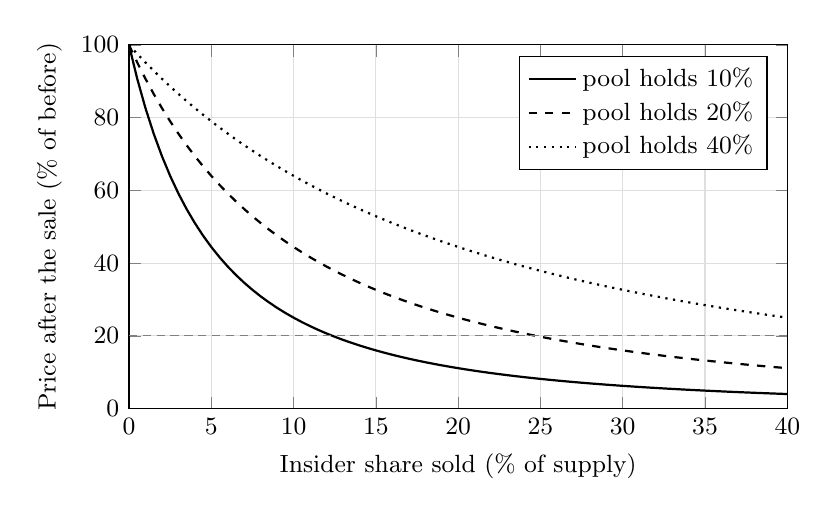
\begin{tikzpicture}
\begin{axis}[width=0.82\linewidth, height=6.2cm, xlabel={Insider share sold (\% of supply)}, ylabel={Price after the sale (\% of before)}, xmin=0, xmax=40, ymin=0, ymax=100, grid=major, grid style={gray!25}, legend pos=north east, legend cell align=left, tick label style={font=\small}, label style={font=\small}, legend style={font=\small}]
\addplot[solid, thick] coordinates {(0.0000,100.0000) (0.5000,90.7029) (1.0000,82.6446) (1.5000,75.6144) (2.0000,69.4444) (2.5000,64.0000) (3.0000,59.1716) (3.5000,54.8697) (4.0000,51.0204) (4.5000,47.5624) (5.0000,44.4444) (5.5000,41.6233) (6.0000,39.0625) (6.5000,36.7309) (7.0000,34.6021) (7.5000,32.6531) (8.0000,30.8642) (8.5000,29.2184) (9.0000,27.7008) (9.5000,26.2985) (10.0000,25.0000) (10.5000,23.7954) (11.0000,22.6757) (11.5000,21.6333) (12.0000,20.6612) (12.5000,19.7531) (13.0000,18.9036) (13.5000,18.1077) (14.0000,17.3611) (14.5000,16.6597) (15.0000,16.0000) (15.5000,15.3787) (16.0000,14.7929) (16.5000,14.2399) (17.0000,13.7174) (17.5000,13.2231) (18.0000,12.7551) (18.5000,12.3115) (19.0000,11.8906) (19.5000,11.4910) (20.0000,11.1111) (20.5000,10.7498) (21.0000,10.4058) (21.5000,10.0781) (22.0000,9.7656) (22.5000,9.4675) (23.0000,9.1827) (23.5000,8.9107) (24.0000,8.6505) (24.5000,8.4016) (25.0000,8.1633) (25.5000,7.9349) (26.0000,7.7160) (26.5000,7.5061) (27.0000,7.3046) (27.5000,7.1111) (28.0000,6.9252) (28.5000,6.7465) (29.0000,6.5746) (29.5000,6.4092) (30.0000,6.2500) (30.5000,6.0966) (31.0000,5.9488) (31.5000,5.8064) (32.0000,5.6689) (32.5000,5.5363) (33.0000,5.4083) (33.5000,5.2847) (34.0000,5.1653) (34.5000,5.0499) (35.0000,4.9383) (35.5000,4.8303) (36.0000,4.7259) (36.5000,4.6248) (37.0000,4.5269) (37.5000,4.4321) (38.0000,4.3403) (38.5000,4.2512) (39.0000,4.1649) (39.5000,4.0812) (40.0000,4.0000)}; \addlegendentry{pool holds 10\%}
\addplot[dashed, thick] coordinates {(0.0000,100.0000) (0.5000,95.1814) (1.0000,90.7029) (1.5000,86.5333) (2.0000,82.6446) (2.5000,79.0123) (3.0000,75.6144) (3.5000,72.4310) (4.0000,69.4444) (4.5000,66.6389) (5.0000,64.0000) (5.5000,61.5148) (6.0000,59.1716) (6.5000,56.9598) (7.0000,54.8697) (7.5000,52.8926) (8.0000,51.0204) (8.5000,49.2459) (9.0000,47.5624) (9.5000,45.9638) (10.0000,44.4444) (10.5000,42.9992) (11.0000,41.6233) (11.5000,40.3124) (12.0000,39.0625) (12.5000,37.8698) (13.0000,36.7309) (13.5000,35.6427) (14.0000,34.6021) (14.5000,33.6064) (15.0000,32.6531) (15.5000,31.7397) (16.0000,30.8642) (16.5000,30.0244) (17.0000,29.2184) (17.5000,28.4444) (18.0000,27.7008) (18.5000,26.9860) (19.0000,26.2985) (19.5000,25.6369) (20.0000,25.0000) (20.5000,24.3865) (21.0000,23.7954) (21.5000,23.2254) (22.0000,22.6757) (22.5000,22.1453) (23.0000,21.6333) (23.5000,21.1389) (24.0000,20.6612) (24.5000,20.1995) (25.0000,19.7531) (25.5000,19.3213) (26.0000,18.9036) (26.5000,18.4992) (27.0000,18.1077) (27.5000,17.7285) (28.0000,17.3611) (28.5000,17.0050) (29.0000,16.6597) (29.5000,16.3249) (30.0000,16.0000) (30.5000,15.6847) (31.0000,15.3787) (31.5000,15.0815) (32.0000,14.7929) (32.5000,14.5125) (33.0000,14.2399) (33.5000,13.9750) (34.0000,13.7174) (34.5000,13.4669) (35.0000,13.2231) (35.5000,12.9860) (36.0000,12.7551) (36.5000,12.5303) (37.0000,12.3115) (37.5000,12.0983) (38.0000,11.8906) (38.5000,11.6882) (39.0000,11.4910) (39.5000,11.2986) (40.0000,11.1111)}; \addlegendentry{pool holds 20\%}
\addplot[dotted, thick] coordinates {(0.0000,100.0000) (0.5000,97.5461) (1.0000,95.1814) (1.5000,92.9017) (2.0000,90.7029) (2.5000,88.5813) (3.0000,86.5333) (3.5000,84.5554) (4.0000,82.6446) (4.5000,80.7979) (5.0000,79.0123) (5.5000,77.2854) (6.0000,75.6144) (6.5000,73.9970) (7.0000,72.4310) (7.5000,70.9141) (8.0000,69.4444) (8.5000,68.0200) (9.0000,66.6389) (9.5000,65.2995) (10.0000,64.0000) (10.5000,62.7389) (11.0000,61.5148) (11.5000,60.3261) (12.0000,59.1716) (12.5000,58.0499) (13.0000,56.9598) (13.5000,55.9001) (14.0000,54.8697) (14.5000,53.8675) (15.0000,52.8926) (15.5000,51.9438) (16.0000,51.0204) (16.5000,50.1214) (17.0000,49.2459) (17.5000,48.3932) (18.0000,47.5624) (18.5000,46.7529) (19.0000,45.9638) (19.5000,45.1945) (20.0000,44.4444) (20.5000,43.7129) (21.0000,42.9992) (21.5000,42.3029) (22.0000,41.6233) (22.5000,40.9600) (23.0000,40.3124) (23.5000,39.6801) (24.0000,39.0625) (24.5000,38.4592) (25.0000,37.8698) (25.5000,37.2939) (26.0000,36.7309) (26.5000,36.1807) (27.0000,35.6427) (27.5000,35.1166) (28.0000,34.6021) (28.5000,34.0988) (29.0000,33.6064) (29.5000,33.1246) (30.0000,32.6531) (30.5000,32.1915) (31.0000,31.7397) (31.5000,31.2974) (32.0000,30.8642) (32.5000,30.4400) (33.0000,30.0244) (33.5000,29.6173) (34.0000,29.2184) (34.5000,28.8275) (35.0000,28.4444) (35.5000,28.0689) (36.0000,27.7008) (36.5000,27.3399) (37.0000,26.9860) (37.5000,26.6389) (38.0000,26.2985) (38.5000,25.9645) (39.0000,25.6369) (39.5000,25.3155) (40.0000,25.0000)}; \addlegendentry{pool holds 40\%}
\addplot[gray, densely dashed] coordinates {(0,20) (40,20)};
\end{axis}
\end{tikzpicture}
\caption{Price after an insider sale in a constant-product pool, by the pool's share of supply (Proposition 1). The grey line marks an 80\% drop. Computed by Appendix~B.}
\label{fig:exit}
\end{figure}


An 80\% price drop needs an insider share of only 12.4\% when the pool holds 10\% of supply, and 49.4\% when it holds 40\%. The v1 cap at 30\% is too lax for thin pools and arguably too strict for deep ones. The same objection applies to the top-ten-holders factor. Concentrated-liquidity pools need the simulated version of this calculation (Section 5.2), but the direction of the result is the same.

\textbf{F7. The caps are cliffs.} \emph{Confirmed.} Caps were applied after normalisation; in the F5 example an insider share of 29.9\% scores 79 and 30.1\% scores 30.

\textbf{F8. Absolute thresholds are not portable across launchpads.} \emph{Confirmed and wider than stated.} Not only ArcPad: lift.fun, Tolly and Argus also launch the whole supply as a single-sided position, so the pool's USDC starts at zero and every such launch began under the 1,000 USDC cap and with zero depth points. For V4 pools the ``liquidity'' was net swap flow, so the depth factor measured demand. Sashimi produced no graduation in the observation window, so its treatment could not be checked.

\textbf{F9. Contract and hook risk is disclosed but not scored.} \emph{Confirmed for the audited version, partly addressed later.} The 1 October code had no sell simulation, no tax read and no fee-mutability check. On 7 October v1 began reading each hook's current taxes, scored round-trip costs (weight 5) and capped a sell tax of 20\% or more at 35. It never simulated a sale and never asked whether a fee could change.

\textbf{F10. Several inputs cost only gas to fake.} \emph{Confirmed.} Shared-funder detection followed one hop (the last USDC sender), looked only at buyers in the first 20 blocks, and ignored hubs by skipping to the previous sender rather than ending the path.

\textbf{F11. The wallet labels reward luck and insiders.} \emph{Partly right.} The window (24 hours, at least five launches) is as stated, but the code required at least 55\% of launches won rather than more than half, and counted unsold tokens at the current price. At five and ten launches the two rules coincide, so the false-positive rates quoted for five launches (16.3\%, 23.5\% and 31.7\% at \emph{q} of 0.30, 0.35 and 0.40) stand; at 15, 30 and 40 launches the code's rule is stricter (Appendix B). Marking unsold tokens to the current price makes a ``win'' depend on the moment the label was computed.

\begin{figure}[t]
\centering
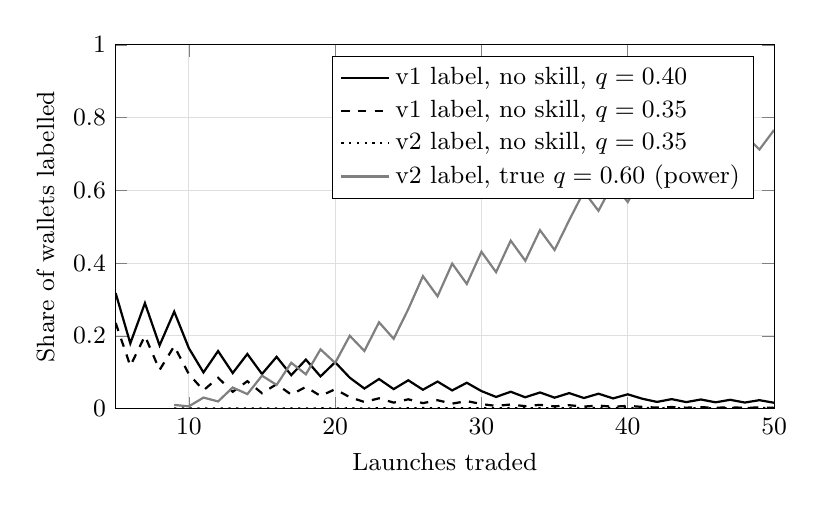
\begin{tikzpicture}
\begin{axis}[width=0.82\linewidth, height=6.2cm, xlabel={Launches traded}, ylabel={Share of wallets labelled}, xmin=5, xmax=50, ymin=0, ymax=1, grid=major, grid style={gray!25}, legend pos=north east, legend cell align=left, tick label style={font=\small}, label style={font=\small}, legend style={font=\small}]
\addplot[thick] coordinates {(5.0000,0.3174) (6.0000,0.1792) (7.0000,0.2898) (8.0000,0.1737) (9.0000,0.2666) (10.0000,0.1662) (11.0000,0.0994) (12.0000,0.1582) (13.0000,0.0977) (14.0000,0.1501) (15.0000,0.0950) (16.0000,0.1423) (17.0000,0.0919) (18.0000,0.1347) (19.0000,0.0885) (20.0000,0.1275) (21.0000,0.0849) (22.0000,0.0551) (23.0000,0.0813) (24.0000,0.0535) (25.0000,0.0778) (26.0000,0.0518) (27.0000,0.0743) (28.0000,0.0499) (29.0000,0.0710) (30.0000,0.0481) (31.0000,0.0320) (32.0000,0.0463) (33.0000,0.0310) (34.0000,0.0444) (35.0000,0.0300) (36.0000,0.0426) (37.0000,0.0290) (38.0000,0.0409) (39.0000,0.0280) (40.0000,0.0392) (41.0000,0.0270) (42.0000,0.0183) (43.0000,0.0260) (44.0000,0.0178) (45.0000,0.0250) (46.0000,0.0172) (47.0000,0.0241) (48.0000,0.0166) (49.0000,0.0231) (50.0000,0.0160)}; \addlegendentry{v1 label, no skill, $q=0.40$}
\addplot[thick, dashed] coordinates {(5.0000,0.2352) (6.0000,0.1174) (7.0000,0.1998) (8.0000,0.1061) (9.0000,0.1717) (10.0000,0.0949) (11.0000,0.0501) (12.0000,0.0846) (13.0000,0.0462) (14.0000,0.0753) (15.0000,0.0422) (16.0000,0.0671) (17.0000,0.0383) (18.0000,0.0597) (19.0000,0.0347) (20.0000,0.0532) (21.0000,0.0313) (22.0000,0.0180) (23.0000,0.0283) (24.0000,0.0164) (25.0000,0.0255) (26.0000,0.0150) (27.0000,0.0229) (28.0000,0.0136) (29.0000,0.0206) (30.0000,0.0124) (31.0000,0.0073) (32.0000,0.0112) (33.0000,0.0066) (34.0000,0.0102) (35.0000,0.0061) (36.0000,0.0092) (37.0000,0.0055) (38.0000,0.0083) (39.0000,0.0050) (40.0000,0.0075) (41.0000,0.0046) (42.0000,0.0027) (43.0000,0.0042) (44.0000,0.0025) (45.0000,0.0038) (46.0000,0.0023) (47.0000,0.0034) (48.0000,0.0021) (49.0000,0.0031) (50.0000,0.0019)}; \addlegendentry{v1 label, no skill, $q=0.35$}
\addplot[thick, dotted] coordinates {(9.0000,0.0001) (10.0000,0.0000) (11.0000,0.0002) (12.0000,0.0001) (13.0000,0.0003) (14.0000,0.0001) (15.0000,0.0005) (16.0000,0.0002) (17.0000,0.0006) (18.0000,0.0003) (19.0000,0.0007) (20.0000,0.0003) (21.0000,0.0007) (22.0000,0.0003) (23.0000,0.0008) (24.0000,0.0004) (25.0000,0.0008) (26.0000,0.0015) (27.0000,0.0008) (28.0000,0.0015) (29.0000,0.0008) (30.0000,0.0014) (31.0000,0.0008) (32.0000,0.0014) (33.0000,0.0007) (34.0000,0.0013) (35.0000,0.0007) (36.0000,0.0012) (37.0000,0.0020) (38.0000,0.0012) (39.0000,0.0019) (40.0000,0.0011) (41.0000,0.0018) (42.0000,0.0010) (43.0000,0.0016) (44.0000,0.0009) (45.0000,0.0015) (46.0000,0.0009) (47.0000,0.0014) (48.0000,0.0021) (49.0000,0.0013) (50.0000,0.0019)}; \addlegendentry{v2 label, no skill, $q=0.35$}
\addplot[thick, gray] coordinates {(9.0000,0.0101) (10.0000,0.0060) (11.0000,0.0302) (12.0000,0.0196) (13.0000,0.0579) (14.0000,0.0398) (15.0000,0.0905) (16.0000,0.0651) (17.0000,0.1260) (18.0000,0.0942) (19.0000,0.1629) (20.0000,0.1256) (21.0000,0.2002) (22.0000,0.1584) (23.0000,0.2373) (24.0000,0.1919) (25.0000,0.2735) (26.0000,0.3642) (27.0000,0.3087) (28.0000,0.3986) (29.0000,0.3427) (30.0000,0.4311) (31.0000,0.3752) (32.0000,0.4618) (33.0000,0.4064) (34.0000,0.4908) (35.0000,0.4361) (36.0000,0.5181) (37.0000,0.5968) (38.0000,0.5439) (39.0000,0.6193) (40.0000,0.5681) (41.0000,0.6404) (42.0000,0.5910) (43.0000,0.6601) (44.0000,0.6126) (45.0000,0.6786) (46.0000,0.6329) (47.0000,0.6960) (48.0000,0.7525) (49.0000,0.7123) (50.0000,0.7660)}; \addlegendentry{v2 label, true $q=0.60$ (power)}
\end{axis}
\end{tikzpicture}
\caption{Chance that a wallet earns a skill label, by launches traded: v1's ``profitable trader'' rule as implemented (at least 55\% of launches won) for wallets with no skill, and the v2 rule of Section~5.8 for wallets with no skill and with a true win rate of 0.60. Computed by Appendix~B.}
\label{fig:labels}
\end{figure}


The label is also confounded with the insider signal. Consistent winners on launchpads are disproportionately creators and snipers {[}11{]}. A factor that awards points when ``wallets with a winning record are holding'' may be awarding points for the presence of the wallets the insider factor is meant to penalise. Independent evidence finds the signal weak and non-monotonic {[}10{]}, and following such wallets loses money after price impact {[}12{]}.

\textbf{F12. There is no uncertainty, validation or version history.} \emph{Confirmed.} The code scored a token from its first block. The repository holds the code's history, but no changelog or backtest was published.

\subsubsection{3.4 What v1 gets right}\label{what-v1-gets-right}

Four choices in v1 are sound and are kept. Deal-breakers are non-compensatory in spirit. Pool and launchpad contracts are excluded from holder counts. Funding-source linkage is the right first step in entity resolution. The ``base rates'' panel, which shows how many earlier launches at the same market cap went on to double, is an outcome-conditioned frequency and is the seed of the calibrated design in Section 5.

\subsubsection{3.5 Summary}\label{summary}

{\def\LTcaptype{none} % do not increment counter
\begin{longtable}[]{@{}
  >{\raggedright\arraybackslash}p{(\linewidth - 8\tabcolsep) * \real{0.2000}}
  >{\raggedright\arraybackslash}p{(\linewidth - 8\tabcolsep) * \real{0.2000}}
  >{\raggedright\arraybackslash}p{(\linewidth - 8\tabcolsep) * \real{0.2000}}
  >{\raggedright\arraybackslash}p{(\linewidth - 8\tabcolsep) * \real{0.2000}}
  >{\raggedright\arraybackslash}p{(\linewidth - 8\tabcolsep) * \real{0.2000}}@{}}
\toprule\noalign{}
\begin{minipage}[b]{\linewidth}\raggedright
\#
\end{minipage} & \begin{minipage}[b]{\linewidth}\raggedright
Finding
\end{minipage} & \begin{minipage}[b]{\linewidth}\raggedright
Status against the code
\end{minipage} & \begin{minipage}[b]{\linewidth}\raggedright
Evidence
\end{minipage} & \begin{minipage}[b]{\linewidth}\raggedright
Addressed in
\end{minipage} \\
\midrule\noalign{}
\endhead
\bottomrule\noalign{}
\endlastfoot
F1 & Weights sum to 90 & Partly right: the score was normalised & Code; arithmetic & 5.5 \\
F2 & No estimand & Confirmed & Code and page & 5.1 \\
F3 & Structure and activity are summed & Confirmed (44.4\% with wallet records, 37.5\% without) & Code & 5.7 \\
F4 & Momentum is procyclical and reflexive & Confirmed & Code; {[}10, 11, 12, 35{]} & 5.7, 6 \\
F5 & Compensation yields ``Strong'' with 89\% exit impact & Confirmed; score 85, not 76.3 & Code; worked example & 5.5 \\
F6 & Concentration ignores pool depth & Confirmed & Code; Proposition 1 & 5.2 \\
F7 & Caps are cliffs & Confirmed & Code; {[}33{]} & 5.5 \\
F8 & Dollar thresholds are launchpad-dependent & Confirmed for four launchpads, not one & Code; launch transactions & 5.2 \\
F9 & Hook and fee risk unscored & Confirmed on 1 October; taxes scored from 7 October, still no simulation & Code history & 5.2 \\
F10 & Sybil-cheap inputs & Confirmed: one hop & Code; {[}15, 21{]} & 5.3, 6 \\
F11 & Labels reward luck and insiders & Partly right: 55\% rule, marked to market & Code; binomial calculation & 5.8 \\
F12 & No uncertainty or validation & Confirmed & Code; absence & 5.6, 7, 10 \\
\end{longtable}
}

\subsection{4. Design requirements and threat model}\label{design-requirements-and-threat-model}

\subsubsection{4.1 Requirements}\label{requirements}

The audit yields eight requirements. Each is stated so that a design either meets it or does not.

{\def\LTcaptype{none} % do not increment counter
\begin{longtable}[]{@{}
  >{\raggedright\arraybackslash}p{(\linewidth - 4\tabcolsep) * \real{0.3333}}
  >{\raggedright\arraybackslash}p{(\linewidth - 4\tabcolsep) * \real{0.3333}}
  >{\raggedright\arraybackslash}p{(\linewidth - 4\tabcolsep) * \real{0.3333}}@{}}
\toprule\noalign{}
\begin{minipage}[b]{\linewidth}\raggedright
\#
\end{minipage} & \begin{minipage}[b]{\linewidth}\raggedright
Requirement
\end{minipage} & \begin{minipage}[b]{\linewidth}\raggedright
Test
\end{minipage} \\
\midrule\noalign{}
\endhead
\bottomrule\noalign{}
\endlastfoot
R1 & Estimand & Every published number names an event, a horizon, a unit and a resolution rule \\
R2 & Separation & Structure and market activity are never summed; price momentum cannot raise the headline \\
R3 & Non-compensation & No amount of good news on one channel offsets a fatal condition on another \\
R4 & Venue invariance & Quantities are computed against the actual pool, not against fixed dollar thresholds \\
R5 & Honest uncertainty & Outputs carry intervals, and the system abstains when evidence is thin \\
R6 & Incentive alignment & The cheapest way to raise the score is to reduce the risk it measures \\
R7 & Reproducibility & The score is a deterministic function of finalized chain state and a versioned specification \\
R8 & Accountability & Forecasts are committed before outcomes and scored in public; there are no manual overrides \\
\end{longtable}
}

R6 follows Kleinberg and Raghavan's distinction between gaming and improvement {[}34{]}. R8 carries the four-input rule of {[}4{]} into scoring: the platform decides nothing on a user's behalf, and anything it asserts can be checked.

\subsubsection{4.2 Adversary}\label{adversary}

The adversary is a token creator with colluders. The adversary knows the full specification, as the design assumes no secrecy. The adversary controls any number of addresses, since an address on Arc costs cents of USDC gas. The adversary has a capital budget \emph{b}, can prepare in advance by ageing and funding wallets, can deploy any contract or hook the launchpad allows, and can trade with itself.

The adversary has three goals. The first is to raise the score while keeping the ability to extract buyers' funds. The second is to lower a competitor's score, for example by sending dust to make unrelated wallets look linked. The third is to poison the outcome data on which calibration and reputation rest.

Out of scope are compromise of DryDock's infrastructure, validator-level attacks on Arc, off-chain persuasion, and anything requiring legal identity.

\subsubsection{4.3 The platform as a party}\label{the-platform-as-a-party}

The design does not ask users to trust the platform's reported accuracy. It makes that accuracy independently computable (Section 10).

\subsubsection{4.4 Properties of Arc that shape the design}\label{properties-of-arc-that-shape-the-design}

\begin{itemize}
\tightlist
\item
  \textbf{Finality.} Arc finalizes blocks deterministically in under a second {[}57{]}. Scores are computed at a finalized block height, and no reorganisation handling is needed.
\item
  \textbf{Gas in USDC.} Identity creation is nearly free, so any count of addresses is worthless as evidence (F10).
\item
  \textbf{A young chain.} Wallet age on Arc is at most a few weeks. Seniority evidence must come from elsewhere, for example the same address's history on other EVM chains, and must be treated as weak.
\item
  \textbf{Issuer blocklist.} Arc enforces a USDC blocklist {[}2{]}. A sale can fail for reasons outside the token contract, so tradability is tested by simulation, not inferred from code.
\item
  \textbf{Planned confidential transfers.} Circle has described opt-in privacy for Arc {[}57{]}. If transfer amounts become hidden for a token, balance-based features are unobservable and the system must abstain for it.
\end{itemize}

\subsection{5. The protocol}\label{the-protocol}

The protocol publishes three layers and never adds them together. Layer 1 is facts computed by simulation. Layer 2 is forecasts of defined events, calibrated against outcomes. Layer 3 is a description of market activity that cannot move the score.

\begin{figure}[t]
\centering
\begin{tikzpicture}[every node/.style={font=\small}, box/.style={draw, rounded corners=2pt, align=center, minimum height=11mm, inner sep=4pt, text width=40mm}, arrow/.style={-{Stealth[length=2mm]}}]
\node[box, text width=24mm] (state) at (0,-2.2) {Arc state at a finalized block $h$};
\node[box] (facts) at (4.6,0) {Layer 1: facts by simulation (floor, losses, friction)};
\node[box] (prob) at (4.6,-2.2) {Layer 2: event probabilities, in shadow until the gates pass};
\node[box] (panel) at (4.6,-4.4) {Layer 3: market panel (shown, never an input)};
\node[box, text width=33mm] (record) at (11.6,-1.1) {Forecast record};
\node[box, text width=33mm] (root) at (11.6,-2.9) {Merkle root posted to Arc};
\node[box, text width=33mm] (resolve) at (11.6,-4.7) {Resolution at $h+H$ from chain state};
\node[box, text width=33mm] (board) at (11.6,-6.5) {Scoreboard of committed records};
\draw[arrow] (state.east) -- ++(0.5,0) |- (facts.west);
\draw[arrow] (state.east) -- (prob.west);
\draw[arrow] (state.east) -- ++(0.5,0) |- (panel.west);
\draw[arrow] (facts.east) -- (record.west);
\draw[arrow] ($(prob.east)+(0,0.3)$) -- (record.west);
\draw[arrow] (record) -- (root);
\draw[arrow] (root) -- (resolve);
\draw[arrow] (resolve) -- (board);
\draw[arrow, dashed] (board.west) -- ++(-1.2,0) node[below, font=\footnotesize] {recalibration} |- ($(prob.east)+(0,-0.3)$);
\end{tikzpicture}
\caption{The v2 pipeline. One block feeds three layers; only Layers 1 and 2 enter the record, and the market panel has no path into it. The dashed loop is the only route by which outcomes change later forecasts.}
\label{fig:pipeline}
\end{figure}


The market panel receives the same block but has no arrow into the score. The loop at the bottom is the only path by which outcomes change later forecasts.

\subsubsection{5.1 Estimands and resolution rules}\label{estimands-and-resolution-rules}

Every forecast is issued at a finalized block \emph{h} for a horizon \emph{H}. The primary horizon is 24 hours; 1 hour and 7 days are secondary. All quantities refer to a \textbf{reference position}: 100 USDC of the token bought at \emph{h} through the token's main pool.

Let \emph{q} be the tokens that purchase returns, and let \emph{Q(q)} be the USDC returned by selling them through the pool's own code, including fees and hooks. If the sale reverts, \emph{Q} is zero. The round-trip recovery is

\[
\rho_h = \frac{Q_h(q)}{100}
\]

Three \textbf{structural events} are defined on the interval from \emph{h} to \emph{h + H}. Each is an on-chain occurrence that any two archive nodes will agree on. None requires a judgement about intent.

{\def\LTcaptype{none} % do not increment counter
\begin{longtable}[]{@{}
  >{\raggedright\arraybackslash}p{(\linewidth - 4\tabcolsep) * \real{0.3333}}
  >{\raggedright\arraybackslash}p{(\linewidth - 4\tabcolsep) * \real{0.3333}}
  >{\raggedright\arraybackslash}p{(\linewidth - 4\tabcolsep) * \real{0.3333}}@{}}
\toprule\noalign{}
\begin{minipage}[b]{\linewidth}\raggedright
Event
\end{minipage} & \begin{minipage}[b]{\linewidth}\raggedright
Channel
\end{minipage} & \begin{minipage}[b]{\linewidth}\raggedright
Resolution rule
\end{minipage} \\
\midrule\noalign{}
\endhead
\bottomrule\noalign{}
\endlastfoot
E\_T & Tradability & The reference position cannot be sold, or a privileged state change (fee, pause, blocklist, mint, upgrade) lowers its simulated recovery by 20 points or more \\
E\_L & Liquidity & Position owners withdraw at least 50\% of the quote-side liquidity present at \emph{h} \\
E\_I & Insider exit & The pessimistic insider set (Section 5.3) net-sells at least 50\% of the tokens it held at \emph{h} \\
\end{longtable}
}

A fourth, all-cause endpoint is used only in the market panel: \textbf{severe loss}, meaning the reference position returns 20 USDC or less at \emph{h + H}. It mixes structural failure with ordinary loss of interest, which is why it is kept out of the score.

The thresholds 20 points, 50\% and 20 USDC are definitional. They fix what is being forecast. They are not tuned to make results look better, and Section 7 reports sensitivity to them.

\subsubsection{5.2 Layer 1: facts by simulation}\label{layer-1-facts-by-simulation}

For each channel the system simulates the worst event available at block \emph{h} and then sells the reference position. This is done with state-override calls against the pool at \emph{h}, so fees, hooks, tick liquidity and single-sided ranges are handled by the pool's own code. No dollar threshold is involved (R4).

\begin{itemize}
\tightlist
\item
  \textbf{Tradability.} Set every privileged parameter to the worst value the code permits without a timelock longer than \emph{H}. If the code is unverified, upgradeable without delay, or otherwise unbounded, the recovery is taken as zero and flagged ``unbounded''.
\item
  \textbf{Liquidity.} Remove every liquidity position whose owner can withdraw within \emph{H}. Burned positions and positions in a recognised locker that unlocks after \emph{h + H} stay.
\item
  \textbf{Insider exit.} Sell the full balance of the insider set, once for the lower-bound set and once for the pessimistic set.
\end{itemize}

Write the recovery of the reference position after event \emph{k} as ρ with superscript \emph{k}. The \textbf{loss given event} and the \textbf{structural floor} are

\[
\ell_k = 1 - \rho_h^{(k)}, \qquad \Phi_h = 100 \cdot \min_{k \in \{T, L, I\}} \rho_h^{(k)}
\]

The floor reads directly: ``in the worst single structural event available now, 100 USDC becomes Φ''. Because the insider set is an interval, so is the floor. The baseline cost of entering and leaving with no event, 1 minus ρ, is reported beside it as friction.

The floor answers F6, F8 and F9 at once. It is pool-relative by construction. It needs no liquidity threshold. A punitive or mutable sell fee appears as a low tradability recovery.

\subsubsection{5.3 Entity resolution as an identified set}\label{entity-resolution-as-an-identified-set}

Common control cannot be observed, so the system reports bounds (Section 2.4).

\textbf{The lower-bound set} contains the creator and every wallet tied to it by positive evidence: funding within \emph{d} hops through non-hub addresses, purchases in the creation block, receipt of the token by transfer before a first purchase, or proceeds that converge on a common address. Bridges, exchange wallets and launchpad routers are hubs. They are listed in a public registry and end a funding path.

\textbf{The pessimistic set} adds every holder that cannot show independence. Independence requires all three of: an address history that predates the token by a set margin, on Arc or on another EVM chain; a first purchase outside the launch window; and funding that does not trace only to fresh unlabelled addresses. The burden of proof sits on independence.

Links are created only by value the linked wallet acted on. An unsolicited inbound transfer never creates a link. This closes the dust-griefing attack of Section 4.2.

\emph{Proposition 2 (Sybil monotonicity).} Suppose the adversary redistributes a fixed insider holding among any number of newly created addresses and inserts any number of newly created funding intermediaries. The token balance of the pessimistic set, and therefore the pessimistic insider loss and the lower end of the floor, do not change.

\emph{Proof.} A newly created address fails the history test and belongs to the pessimistic set whether or not it is linked. Redistribution conserves the total balance. ∎

The adversary can shrink the pessimistic set only by using addresses with real history, which are scarce and take time to build, or by actually distributing tokens to independent holders. The second is improvement, not gaming (R6).

The weakness is stated plainly. On a three-week-old chain most honest buyers also lack history, so the pessimistic bound is wide for almost every launch. The interval is still correct, and the forecasting layer learns from outcomes how much weight each end deserves.

\subsubsection{5.4 What the forecasts condition on}\label{what-the-forecasts-condition-on}

Each channel has its own feature block. Every feature has one direction: more of it can only raise the forecast probability.

{\def\LTcaptype{none} % do not increment counter
\begin{longtable}[]{@{}
  >{\raggedright\arraybackslash}p{(\linewidth - 4\tabcolsep) * \real{0.3333}}
  >{\raggedright\arraybackslash}p{(\linewidth - 4\tabcolsep) * \real{0.3333}}
  >{\raggedright\arraybackslash}p{(\linewidth - 4\tabcolsep) * \real{0.3333}}@{}}
\toprule\noalign{}
\begin{minipage}[b]{\linewidth}\raggedright
Channel
\end{minipage} & \begin{minipage}[b]{\linewidth}\raggedright
Risk features
\end{minipage} & \begin{minipage}[b]{\linewidth}\raggedright
Protective facts
\end{minipage} \\
\midrule\noalign{}
\endhead
\bottomrule\noalign{}
\endlastfoot
Tradability & Privileged roles present; maximum settable fee; hook permissions that alter swap amounts; unverified or upgradeable code & Roles renounced; fee parameters immutable; timelock longer than the horizon \\
Liquidity & Share withdrawable within the horizon; owner is an ordinary wallet; unlock inside the horizon & Position burned; recognised locker with later unlock \\
Insider exit & Insider loss at both bounds; share of public USDC the insiders can extract; recent insider net selling; bundled creation-block buys; creator cluster's prior event rate; wash share & Insider tokens in a vesting or timelock contract \\
\end{longtable}
}

Protective facts are irreversible or time-locked commitments. They cannot be faked without being done, and doing them lowers the risk (R6). Wash share enters as a risk feature only: fabricated activity predicts later extraction {[}13{]}, and genuine activity earns no credit here.

Creator history uses a shrunk estimate. A creator cluster's prior event rate is a Beta-Binomial posterior with a launchpad-level prior {[}42{]}. A new creator gets the prior, neither penalty nor credit, which matches the treatment of fresh identities in {[}4{]}. Launches are weighted by public capital at risk so that many tiny self-traded tokens cannot manufacture a record.

\subsubsection{5.5 Model and aggregation}\label{model-and-aggregation}

Each channel probability is a discrete-time hazard with monotone components:

\[
\operatorname{logit} \pi_k(h, H) = \alpha_{k,\mathrm{pad}} + s_k(\mathrm{age}) + \sum_j m_{kj}(x_j), \qquad m_{kj} \ \text{non-decreasing}
\]

The launchpad intercepts are partially pooled toward a common mean, so a launchpad with little history borrows strength from the others {[}60{]}. The age term is a baseline hazard. Tokens that have not reached their horizon are right-censored and handled as in survival analysis {[}43{]}, and repeated forecasts for one token are evaluated at fixed ages by landmarking {[}44{]}.

Monotonicity serves three purposes. Each feature has an interpretable direction. With few outcomes, the constraint is strong regularisation. An adversary cannot find a region where adding risk improves the forecast.

Under independent channel events and multiplicative recoveries, the expected recovery of the reference position is a product. The \textbf{Integrity Score} is that expectation on a 0 to 100 scale:

\[
\mathrm{IS}_h = 100 \prod_{k \in \{T, L, I\}} \bigl(1 - \pi_k \, \ell_k\bigr)
\]

The score has a unit: expected USDC remaining, per 100, after structural events over the horizon. It equals 100 when no event is likely or none would hurt. It falls toward the floor as the worst event becomes certain.

\emph{Proposition 3 (non-compensation).} For every channel \emph{k}, the Integrity Score is at most 100(1 − πₖℓₖ), and it is non-increasing in every π and every ℓ.

\emph{Proof.} Each factor of the product lies in {[}0, 1{]} and is decreasing in its π and ℓ. ∎

No feature outside channel \emph{k} can lift the score above the bound that channel sets. Caps are unnecessary, and there are no cliffs (F5, F7). The independence assumption is tested, not trusted: Section 7 checks whether mean realised recovery matches the score in each score bin.

\subsubsection{5.6 Calibration, uncertainty and staged release}\label{calibration-uncertainty-and-staged-release}

Arc has too little history to estimate probabilities today. The release is therefore staged, and each stage says what it is.

\begin{enumerate}
\def\labelenumi{\arabic{enumi}.}
\tightlist
\item
  \textbf{Stage 0, severity only.} Publish the floor interval, the three losses given event and friction. Publish no probability. This stage needs no outcome data and can ship now.
\item
  \textbf{Stage 1, calibrated channels.} Once the sample-size gates of Section 7.5 are met, publish each π with a Venn-Abers interval {[}31{]}. Recalibrate on a trailing window by isotonic regression {[}27{]} and track coverage with adaptive conformal updates {[}32{]}.
\item
  \textbf{Stage 2, Integrity Score.} Publish the score as the headline only after it passes the ship criteria of Section 7.6 on out-of-time data.
\end{enumerate}

The system abstains in three cases. ``Too early'' applies below a minimum token age or a minimum number of independent trading entities. ``Unobservable'' applies when balances are hidden or code is unbounded. ``Low confidence'' applies when the probability interval is wider than a set width. An abstention is shown as such, never as a low or middling number (F12).

For Stage 0 a letter grade summarises the lower end of the floor: A for 90 or more, B for 75 to 89, C for 50 to 74, D for 20 to 49, E below 20. The bands are presentation only. Each is a statement in USDC, and none is used in any computation.

\subsubsection{5.7 Layer 3: the market panel}\label{layer-3-the-market-panel}

Market activity is shown beside the score and never inside it (R2). Price momentum appears only as a chart.

\begin{itemize}
\tightlist
\item
  \textbf{Net retained public inflow.} USDC paid in by entities outside the pessimistic set, minus USDC they took out. Round-trip volume nets to zero.
\item
  \textbf{Effective participants.} The exponential of the entropy of net-inflow shares, a Hill number {[}56{]}. Splitting one buyer into thirty linked wallets leaves it unchanged.
\item
  \textbf{Wash share.} Volume in closed cycles or matched equal-size round trips, as a share of total volume {[}11, 16{]}, with a flag when swap fees flow back to the creator.
\item
  \textbf{Depth.} Round-trip recovery of a 1,000 USDC position.
\item
  \textbf{Reference-class outcome.} The severe-loss frequency among earlier launches on the same launchpad at a similar age and floor grade, stated as counts.
\end{itemize}

\[
N_{\mathrm{eff}} = \exp\Bigl(-\sum_i s_i \ln s_i\Bigr)
\]

The reference-class line generalises v1's ``base rates''. It is written as a natural frequency, for example ``of N earlier launches like this one, M returned 20 USDC or less per 100 after 24 hours'', because readers reason more accurately from counts than from percentages {[}51{]}.

\subsubsection{5.8 Wallet labels}\label{wallet-labels}

Behavioural labels such as ``bot'' and ``sniper'' describe what a wallet did and stay as descriptions. The skill label changes in four ways.

\begin{enumerate}
\def\labelenumi{\arabic{enumi}.}
\tightlist
\item
  The window is 30 days and at least 20 resolved launches, not 24 hours and five.
\item
  Launches where the wallet belongs to the lower-bound insider set are excluded. Insider profit is not skill.
\item
  A wallet is labelled only if the posterior probability that its win rate exceeds the launchpad baseline by five points is above 0.95, under a Beta prior centred on that baseline {[}42{]}, with false-discovery control across wallets {[}39, 40, 41{]}.
\item
  The label must hold out of sample: assigned on one window, confirmed on the next, as in {[}10{]}.
\end{enumerate}

With a prior of mean 0.35 and weight 20, a wallet with five launches can never qualify, and one with 20 launches needs 15 wins. The false-positive rate stays below 0.2\% at every sample size tested. The cost is power: a wallet with a true 60\% win rate is detected 77\% of the time at 50 launches. Skill takes that long to tell from luck. The label never enters the score.

\subsubsection{5.9 Presentation}\label{presentation}

The token page leads with facts in currency, then the forecast, then the market panel. Verdict words such as ``Strong setup'' are retired. They assert safety in a population where most launches fail, and no data yet show that the top band is safe. The stage of each number is printed beside it.

\subsection{6. Manipulation-resistance analysis}\label{manipulation-resistance-analysis}

Of eleven attacks, v2 removes the payoff of eight by construction and leaves three with a stated residual. The adversary is the one in Section 4.2 and knows the full specification.

\subsubsection{6.1 Attacks}\label{attacks}

{\def\LTcaptype{none} % do not increment counter
\begin{longtable}[]{@{}
  >{\raggedright\arraybackslash}p{(\linewidth - 8\tabcolsep) * \real{0.2000}}
  >{\raggedright\arraybackslash}p{(\linewidth - 8\tabcolsep) * \real{0.2000}}
  >{\raggedright\arraybackslash}p{(\linewidth - 8\tabcolsep) * \real{0.2000}}
  >{\raggedright\arraybackslash}p{(\linewidth - 8\tabcolsep) * \real{0.2000}}
  >{\raggedright\arraybackslash}p{(\linewidth - 8\tabcolsep) * \real{0.2000}}@{}}
\toprule\noalign{}
\begin{minipage}[b]{\linewidth}\raggedright
\#
\end{minipage} & \begin{minipage}[b]{\linewidth}\raggedright
Attack
\end{minipage} & \begin{minipage}[b]{\linewidth}\raggedright
Effect on v1
\end{minipage} & \begin{minipage}[b]{\linewidth}\raggedright
Effect on v2
\end{minipage} & \begin{minipage}[b]{\linewidth}\raggedright
Residual in v2
\end{minipage} \\
\midrule\noalign{}
\endhead
\bottomrule\noalign{}
\endlastfoot
A1 & Split insider holdings across fresh wallets & Lowers top-ten share; lowers insider share if unlinked. Cost: gas & None on the pessimistic bound (Proposition 2) & None \\
A2 & Fund buyers through intermediaries, bridges or exchanges & Defeats the one-hop shared-funder check & Lower bound may miss the link; pessimistic bound unchanged & Wider interval \\
A3 & Use wallets aged in advance & Not needed & Shrinks the pessimistic set & Open; see 6.3 \\
A4 & Wash trade, with fees returned to the creator & Raises demand and momentum, up to 30 points & No credit; raises wash share; net buying lowers the score (Proposition 4) & None \\
A5 & Sit just under a threshold & Avoids each cap at 29.9\% insiders or 1,001 USDC & No thresholds in any computation & None \\
A6 & Rent liquidity by buying with own wallets & 25k USDC appears in a locked pool & The buying wallets hold tokens, so insider loss rises & None \\
A7 & Farm a creator record with one self-pumped launch & 10 points on every later launch & Record is shrunk and weighted by public capital at risk & Small \\
A8 & Flip a privilege after buyers enter & Unscored & Priced in advance by worst-case simulation & Code outside the analyser's reach is scored as unbounded \\
A9 & Send dust to link a competitor's buyers & Possible where funding precedes a known wallet's purchase & Links need value the wallet acted on & None \\
A10 & Mass-launch tiny tokens to bias base rates & Shifts the base-rate panel & Minimum public inflow for inclusion; grouping by creator cluster & Small \\
A11 & Behave until the horizon passes, then exit & Unscored & Rolling forecasts; unlock dates inside 7 days are priced & Open beyond the longest horizon \\
\end{longtable}
}

The cost of A6 under v1 is the round-trip fee on the rented amount. At the 1\% fee tier the launchpads use {[}3{]}, that is about 500 USDC on 25,000, less wherever fees return to the creator. A4 at thirty wallets and 20 USDC each costs about 12 USDC in fees plus gas. Under v1, a few hundred USDC of fees can therefore move 45 of 90 points. These are order-of-magnitude figures from the published rules, not measurements.

\subsubsection{6.2 Two further propositions}\label{two-further-propositions}

\emph{Proposition 4 (no credit for buying pressure).} In a constant-product pool, any net purchase of the token from the pool, by anyone, weakly raises the insider loss given event for a fixed insider balance. Holding the forecast probabilities fixed, it weakly lowers the Integrity Score.

\emph{Proof.} A purchase lowers the pool's token share from \emph{g} to \emph{g′} \textless{} \emph{g}. By Proposition 1 the post-exit price multiple (\emph{g′}/(\emph{g′} + \emph{f}))² is increasing in \emph{g′}, so it falls. If the purchaser is in the insider set, \emph{f} rises as well. The reference recovery after the exit falls in both cases, and the score is non-increasing in that loss (Proposition 3). No feature in Section 5.4 rewards purchases. ∎

Pumping the price is self-defeating under v2. This is the formal content of R2.

\emph{Proposition 5 (routes to a higher floor).} Every action that raises the lower end of the structural floor falls into one of four classes: (a) removing or time-locking a privilege; (b) burning or locking liquidity; (c) burning, locking, selling or genuinely distributing insider tokens; (d) moving insider tokens to addresses that pass the independence test while remaining under common control.

\emph{Proof.} The floor is the minimum of three recoveries. The tradability recovery rises only if the worst reachable privileged state improves, which is (a). The liquidity recovery rises only if the withdrawable share falls, which is (b). The insider recovery rises only if the pessimistic set's sellable balance falls relative to pool depth. Depth rises relative to that balance only through liquidity that is not withdrawable, which is (b) again, since withdrawable liquidity lowers the liquidity recovery. The balance falls only by burn, lock, sale or transfer. A transfer leaves the pessimistic set only if the recipient passes the independence test, which is genuine distribution (c) or aged-wallet control (d). ∎

Classes (a) to (c) reduce what the adversary can extract over the horizon. They are improvement in the sense of {[}34{]}. Class (d) is the only gaming route, and its cost is the cost of manufacturing address history.

\subsubsection{6.3 Residual risks}\label{residual-risks}

\textbf{Aged wallets (A3, class d).} An organised farm can prepare addresses with months of plausible activity. Three countermeasures raise its cost without closing it: the history margin lengthens as Arc matures; co-trading recurrence across launches links wallets that repeatedly appear together; and proceeds that converge on one address link sellers after the fact, which feeds the creator cluster's record for the next launch. The lower and upper bounds are both model inputs, so if aged-wallet attacks become common the fitted weight shifts toward features they cannot move.

\textbf{Opaque code (A8).} Worst-case simulation is only as good as the analysis of what privileged calls can do. Template launchpads make this tractable because hooks and tokens come from a small set of known contracts. Anything else is scored as unbounded, which is conservative and will be wrong for some honest custom tokens.

\textbf{Long cons (A11).} A creator who waits past the longest horizon is outside any forecast the system issues. The score is about a stated window, and the page must say so.

\textbf{Performative drift.} If buyers concentrate on high-score launches, the public USDC in those pools grows, and so does the incentive to exit {[}35{]}. The feature ``share of public USDC the insiders can extract'' tracks this directly, and recalibration on a trailing window follows the shift. The size of the effect is an empirical question that Section 7 measures.

\subsection{7. Validation protocol}\label{validation-protocol}

This section is a pre-registration. It fixes hypotheses, data, baselines, metrics and decision rules before any Arc outcome is examined. Because forecasts are committed on-chain before they resolve (Section 10), the validation is prospective by construction.

\subsubsection{7.1 Hypotheses}\label{hypotheses}

{\def\LTcaptype{none} % do not increment counter
\begin{longtable}[]{@{}
  >{\raggedright\arraybackslash}p{(\linewidth - 4\tabcolsep) * \real{0.3333}}
  >{\raggedright\arraybackslash}p{(\linewidth - 4\tabcolsep) * \real{0.3333}}
  >{\raggedright\arraybackslash}p{(\linewidth - 4\tabcolsep) * \real{0.3333}}@{}}
\toprule\noalign{}
\begin{minipage}[b]{\linewidth}\raggedright
\#
\end{minipage} & \begin{minipage}[b]{\linewidth}\raggedright
Hypothesis
\end{minipage} & \begin{minipage}[b]{\linewidth}\raggedright
Passes when
\end{minipage} \\
\midrule\noalign{}
\endhead
\bottomrule\noalign{}
\endlastfoot
H1 & The facts layer measures severity & Where an event occurs, realised recovery at the event is within 10 points of the loss computed at the last prior forecast, on average \\
H2 & Channel probabilities are calibrated & Out-of-time calibration slope lies in 0.8 to 1.2 and the intercept interval covers zero, for each channel \\
H3 & The forecasts have skill & Brier skill against the launchpad-by-age base rate is positive, and Brier score is lower than recalibrated v1 \\
H4 & Floor grades order risk & Realised mean loss rises monotonically from grade A to grade E \\
H5 & The skill label finds skill & Labelled wallets beat the baseline win rate by five points out of sample, with false discoveries at or below 10\% \\
H6 & Activity factors add no structural signal & Adding v1's demand and momentum values to the channel models does not lower out-of-time log loss \\
\end{longtable}
}

H6 may fail. If it does, the result is reported, and those factors still stay out of the Integrity Score, because the exclusion rests on manipulability (Proposition 4), not on predictive weakness. That decision is declared here so it cannot be revisited after seeing the data.

\subsubsection{7.2 Data and splits}\label{data-and-splits}

The population is every launch on the six launchpads since mainnet. The unit of analysis is a token at a landmark age: 1 minute, 10 minutes, 1 hour, 6 hours and 24 hours after its first trade {[}44{]}. Landmarks stop long-lived tokens from dominating and remove the autocorrelation of block-by-block forecasts.

Splits run forward in calendar time. All tokens from one creator cluster fall in one fold, so that a serial launcher cannot leak between training and test. One full horizon is embargoed between folds {[}45{]}. No feature at block \emph{h} may read state after \emph{h}, a rule the reproducibility check in Section 10 enforces mechanically.

\subsubsection{7.3 Baselines and ablations}\label{baselines-and-ablations}

{\def\LTcaptype{none} % do not increment counter
\begin{longtable}[]{@{}
  >{\raggedright\arraybackslash}p{(\linewidth - 4\tabcolsep) * \real{0.3333}}
  >{\raggedright\arraybackslash}p{(\linewidth - 4\tabcolsep) * \real{0.3333}}
  >{\raggedright\arraybackslash}p{(\linewidth - 4\tabcolsep) * \real{0.3333}}@{}}
\toprule\noalign{}
\begin{minipage}[b]{\linewidth}\raggedright
Code
\end{minipage} & \begin{minipage}[b]{\linewidth}\raggedright
Model
\end{minipage} & \begin{minipage}[b]{\linewidth}\raggedright
Purpose
\end{minipage} \\
\midrule\noalign{}
\endhead
\bottomrule\noalign{}
\endlastfoot
B0 & Event frequency by launchpad and age & The climatological reference for skill scores \\
B1 & v1 score, mapped to probability by isotonic regression on the training fold & The fairest version of the current system \\
B2 & Logistic regression on v1's seven factor values & Tests whether v1's inputs carry signal its weights lose \\
B3 & v2 with address-level holdings in place of entity sets & Value of entity resolution \\
B4 & v2 with raw supply share in place of simulated loss & Value of pool-relative simulation \\
\end{longtable}
}

\subsubsection{7.4 Metrics}\label{metrics}

Accuracy is measured with the Brier and logarithmic scores {[}23, 25{]}, with Murphy's decomposition reported so that reliability and resolution are visible separately {[}24{]}. Calibration is shown as slope, intercept and reliability diagrams with sampling bands {[}29, 30{]}. Discrimination is reported as area under the ROC curve {[}47{]} and, because events are imbalanced, under the precision-recall curve {[}48{]}.

Usefulness is reported as net benefit across decision thresholds {[}49{]}. Interval coverage, abstention rate and grade changes per token-hour measure honesty and stability. For the Integrity Score, mean realised structural recovery is compared with the score in each decile.

Models are compared on paired forecast differences, with standard errors clustered by creator cluster {[}46{]}. Reporting follows the TRIPOD checklist for prediction models {[}50{]}.

\subsubsection{7.5 Sample-size gates}\label{sample-size-gates}

Stage 1 opens when three counts are met: 2,000 resolved landmark forecasts, 500 distinct creator clusters, and 100 events per channel. The reasoning is as follows.

\begin{itemize}
\tightlist
\item
  Estimating an event frequency in one calibration bin to within 5 points at 95\% confidence needs 139 forecasts when the rate is 0.9 and 385 when it is 0.5.
\item
  An ROC area of 0.75 estimated from 2,000 forecasts with 20\% prevalence has a 95\% half-width of 0.029. From 500 forecasts it is 0.059 {[}47{]}.
\item
  One hundred events per channel allows about ten events per fitted degree of freedom in a ten-term monotone model.
\end{itemize}

A launchpad gets its own intercept only after 300 resolved forecasts on it. Before that it uses the pooled estimate and a wider interval.

\subsubsection{7.6 Ship and kill criteria}\label{ship-and-kill-criteria}

All criteria are evaluated on out-of-time data.

\textbf{Ship the Integrity Score as headline when all hold:}

\begin{enumerate}
\def\labelenumi{\arabic{enumi}.}
\tightlist
\item
  H2 passes for every channel.
\item
  H3 passes, with the paired Brier difference against B1 significant at the 5\% level.
\item
  Interval coverage is within 3 points of nominal.
\item
  Each attack A1 to A11, run on a fork or a test launch, fails to raise the score except through class (d) of Proposition 5.
\item
  Realised mean recovery is within 5 points of the score in at least eight of ten deciles.
\end{enumerate}

\textbf{Withdraw or hold back when any holds:}

\begin{enumerate}
\def\labelenumi{\arabic{enumi}.}
\tightlist
\item
  After 5,000 resolved forecasts the score still fails criterion 2. The probabilities are not published, and the product stays at Stage 0.
\item
  In any calendar quarter the calibration slope leaves the range 0.6 to 1.5. The display reverts to Stage 0 until recalibrated.
\item
  H4 fails. The facts layer is then mis-specified, and grades are withdrawn pending revision.
\end{enumerate}

\subsubsection{7.7 Sensitivity analyses}\label{sensitivity-analyses}

Results are re-run with the event thresholds of Section 5.1 moved to (10 points, 30\%, 10 USDC) and (30 points, 70\%, 30 USDC), with a 1,000 USDC reference position, with funding depth \emph{d} from 1 to 4, with history margins of 7, 30 and 90 days, and with the chain's first week excluded. A conclusion that reverses under any of these is reported as fragile.

\subsubsection{7.8 Deviations from the pre-registration}\label{deviations-from-the-pre-registration}

Sections 7.1 to 7.7 are unchanged from the first version of this paper, written before any Arc outcome was examined. What follows lists every way the work reported in Section 8 departs from them, with the reason. None changes a hypothesis, a baseline or a ship or kill criterion.

\begin{itemize}
\tightlist
\item
  \textbf{D1. Retrospective data.} Section 7 assumes forecasts committed before their outcomes. DryDock began committing on 8 October 2026, so the records behind H1 and H4 in Section 8 were recomputed after the fact for launches since 16 September 2026 (the backfill). They were produced by the same code and parameters as committed records, but their outcomes were already on chain when they were computed. They are labelled retrospective everywhere and reported separately from committed records; the pre-registered tests on committed data remain pending.
\item
  \textbf{D2. Funding lookback.} Appendix A.1 set 7 days. Public Arc nodes that accept wide log ranges keep about 42 hours of history, and the archive nodes accept 100- to 10,000-block ranges at low rates, so a 7-day, three-hop trace cannot be computed at forecast time and records would not be reproducible from public infrastructure. The lookback is 86,400 blocks (about 12 hours), every edge of a path inside one window ending at the wallet's first purchase.
\item
  \textbf{D3. Minimum age.} Appendix A.1 set 120 blocks, glossed as about a minute. Arc produces about 1.97 blocks a second, so every record at the 1-minute landmark was two or three blocks short and could never be rated. The minimum age is 60 seconds of block time.
\item
  \textbf{D4. Large insider sets.} Appendix A.2 sells every insider address in turn. Beyond 100 addresses the rest of the set is sold as one block, credited to one seller through a storage override, to stay inside the 50 million gas that public nodes allow per call. In a constant-product pool with retained fees this returns slightly more to the reference position than address-by-address sales would (Appendix B); in Uniswap V3 and V4, where fees sit outside active liquidity, the two are equal up to rounding.
\item
  \textbf{D5. ``Value the linked wallet acted on.''} Section 5.3 states the principle; the implementation needs a rule. A transfer links two wallets only if it carried at least half of what the recipient then spent on its first purchase or forwarded along the path (Appendix A.3).
\item
  \textbf{D6. Address history.} Section 5.3 allows history ``on Arc or on another EVM chain''. Appendix A.1, which governs, does not; the implementation reads Arc transaction counts only. History on other chains would need archive access to each of them.
\item
  \textbf{D7. Population.} Section 7.2 names six launchpads, including Minara. DryDock lists only launchpads whose tokens its swap router can trade; by 8 October 2026 that was lift.fun, Tolly, ArcPad, Argus, Arcora, o1 Launchpad and Sashimi, while Minara's pools pair with native USDC and are not routable. The population is every launch on those seven since 16 September 2026, identified by the launchpad's own contract logs in the creating transaction.
\item
  \textbf{D8. Committed means committed in time.} Section 10.2 does not say how late a commitment may be. A record counts as committed only if its root was posted within 1,200 blocks of its forecast block (Appendix A.1). The committer account was not funded when the runner started, so the first batches are posted late and fall outside the scoreboard.
\item
  \textbf{D9. v1 baselines without wallet records.} B1 and B2 use v1 as it scored before wallet records loaded, without the smart-money factor: that factor needed 24 hours of every holder's trades across all launches and is not reconstructed for past blocks.
\item
  \textbf{D10. Secondary horizons.} Records and resolutions use the 24-hour horizon only. The 1-hour and 7-day horizons are not yet computed.
\item
  \textbf{D11. A sample, not the population, for the backfill.} Section 7.2 takes every launch. Insider sets and resolutions need each token's transfers until 48 hours after its first trade, and public nodes filter logs only by address, so reconstructing them for all 78,244 traded launches meant downloading every Transfer log on Arc since mainnet opened (estimated at more than eight hours for the transfer scan alone over the bandwidth available). The backfill therefore uses a fixed sample: every traded launch of each launchpad with at most 3,000 of them, and 3,000 drawn uniformly from each larger launchpad (Argus and lift.fun) by a seeded hash of the token address (\texttt{backfillSample} in the released code). The sample was fixed before any record was computed. Results are reported per launchpad, where the sample is uniform; pooled figures weight the smaller launchpads more heavily than the population does, and are labelled as sample figures.
\item
  \textbf{D12. Funding stops at contracts.} Section 5.3 ends funding paths at registered hubs only. On Arc, swap routers and pools that are not in the registry (most have no public identification, which the registry requires) receive hundreds of thousands of USDC transfers a day; following their inflows linked a buyer to every other user of the same router and made a single record cost millions of log reads. From method 2.0.2 a path is traced only into accounts without contract code. Wallets funded through one personal contract still share it as an ancestor, and a contract funder fails the history test, so the pessimistic set is unaffected; the lower bound loses the links that ran through contracts.
\item
  \textbf{D13. Valuing a held position.} Appendix A.5 as first implemented sold the reference position's tokens, credited by a storage override, into the pool as it stood at the later block. That pool never received the position's own purchase, so on thin launches the sale found almost no USDC (on Argus V5 the hook rejected the partial fill) and the resolution recorded a near-total loss that had not happened. The first run of the backfill used that rule; it was found by checking grade-A records whose launches had no trades after \emph{h}, which resolved at 0 while their floor was 96. From method 2.0.3 the position is bought at the later block by exact output and sold straight back, and Uniswap V4 tradability reads the pool's positions at the horizon (it had read none). Every record in Section 8 was recomputed under 2.0.3.
\item
  \textbf{D14. Only rated records are resolved.} Appendix A.5 resolves every record. Records that abstain carry no floor and no grade, so their outcomes enter no hypothesis, and resolving them costs as many chain reads as resolving a rated one; with 98\% of records abstaining, the live resolver could not keep up. Both the backfill and, from 12 October 2026, the live runner resolve rated records only; abstaining records are closed without an outcome. The gate counts of Section 8.4 count rated resolutions only.
\end{itemize}

\subsection{8. Implementation and retrospective results}\label{implementation-and-retrospective-results}

This section reports what was built and what the data since mainnet opened show. Every number in it is produced by \texttt{analysis/results.py} from the released dataset (Appendix C); the records were computed by the same code that issues live records, under method 2.0.3. The records behind Sections 8.2 to 8.5 are retrospective (D1): their outcomes were on chain when they were computed.

\subsubsection{8.1 What was built}\label{what-was-built}

DryDock runs Stage 0 (Section 5.6). For each launch it issues a record 1 minute, 10 minutes, 1 hour, 6 hours and 24 hours after the first swap, computing the facts layer by \texttt{eth\_call} simulation at the forecast block with the pool, hook, position managers and token enforcing their own code (Appendix A.2), the two insider sets (Appendix A.3), and the abstentions. Records are batched every 600 blocks under a Merkle root for the ForecastLedger contract (Section 10.2) and resolved after 24 hours (Appendix A.5). The token page shows the floor interval, its grade, friction and the three losses, with later stages shown as gated; v1's number, factors, caps and verdict words are retired, and v1 survives only as the baselines B1 and B2.

The backfill recomputes the same records for past launches. It reads pool events, token transfers and USDC moves from a local store built by scanning public Arc nodes, and everything else (simulation, code, timestamps, transaction counts) from archive nodes at the historical block.

\subsubsection{8.2 Population, sample and records}\label{population-sample-and-records}

Between 16 September and 7 October 2026 the seven launchpads DryDock lists created 202,944 launches, of which 78,223 traded at least once (Table 8). Argus accounts for 89\% of launches. The backfill covers a fixed sample of 9,475 traded launches (D11): every traded launch of Tolly, o1 Launchpad, ArcPad, Arcora and Sashimi, and 3,000 each from Argus and lift.fun. Each received five records, 47,375 in all; none failed to compute and no resolution failed.

{\def\LTcaptype{none} % do not increment counter
\begin{longtable}[]{@{}lllll@{}}
\toprule\noalign{}
Launchpad & Launches & Traded & In the sample & Rated at 24 h \\
\midrule\noalign{}
\endhead
\bottomrule\noalign{}
\endlastfoot
Argus & 180,434 & 56,534 & 3,000 & 176 \\
lift.fun & 18,285 & 18,214 & 3,000 & 1 \\
Tolly & 2,177 & 1,721 & 1,721 & 25 \\
o1 Launchpad & 1,872 & 1,612 & 1,612 & 0 \\
ArcPad & 164 & 130 & 130 & 0 \\
Arcora & 11 & 11 & 11 & 2 \\
Sashimi & 1 & 1 & 1 & 0 \\
\end{longtable}
}

\emph{Table 8. Launches by launchpad, 16 September to 7 October 2026.}

Most records abstain. At each landmark 1,745 are unobservable: the o1 Launchpad, ArcPad and Sashimi token contracts have no verified source, so the registry cannot bound them (Section 5.2), and two lift.fun launches used unregistered code. Of the rest, between 58 (1 minute) and 215 (1 hour) are rated and the others are too early. Too early here almost never means too young: at the 24-hour landmark, 7,455 of the 7,526 too-early records have fewer than 10 holders in total and 3,764 have none. Most launches on Arc are bought by a handful of wallets or by nobody, and the method declines to rate them.

{\def\LTcaptype{none} % do not increment counter
\begin{longtable}[]{@{}llll@{}}
\toprule\noalign{}
Landmark & Rated & Too early & Unobservable \\
\midrule\noalign{}
\endhead
\bottomrule\noalign{}
\endlastfoot
1 minute & 58 & 7,672 & 1,745 \\
10 minutes & 185 & 7,545 & 1,745 \\
1 hour & 215 & 7,515 & 1,745 \\
6 hours & 214 & 7,516 & 1,745 \\
24 hours & 204 & 7,526 & 1,745 \\
\end{longtable}
}

\emph{Table 9. Record states by landmark, sample of 9,475 launches.}

\subsubsection{8.3 Insider sets on a three-week-old chain}\label{insider-sets-on-a-three-week-old-chain}

Section 5.3 warned that the pessimistic set would be wide on a young chain. It is wider than wide. The history margin asks for activity 30 days before the token's creation, and every launch in the population was created within 22 days of mainnet opening. Across records, the share of holders that pass the history margin has a median of 0\% and a mean of 0.9\%. In 63.2\% of records the pessimistic set holds every holder, and the median share of holders in it is 100\%. The lower-bound set, which needs positive evidence, is much smaller: in the worked example of Section 9.1 it is empty while the pessimistic set holds 65 of 75 holders.

The consequence is that, for now, the lower end of the floor mostly answers the question ``what if everyone who holds sold?'' That question is the right worst case when no holder can show independence, and the data below show it predicts outcomes well, but the interval will narrow only as the chain ages and holders accumulate history.

\subsubsection{8.4 Pre-registered tests}\label{pre-registered-tests}

\textbf{H1 (the facts layer measures severity): fails for insider exit; untestable for the other channels.} Among rated records, 70 launches saw an insider exit after a forecast. At their last prior forecast, the mean absolute difference between the realised recovery at the event and the recovery the pessimistic insider exit predicted is 12.7 points, above the 10-point criterion; the median is 4.4. Every error has the same sign: realised recovery was higher than predicted, so the floor erred on the safe side. No tradability or liquidity event occurred in the sample, so H1 cannot be tested for those channels.

\textbf{H4 (grades order realised loss): passes.} Over 876 resolved rated records, the mean loss of the reference position after 24 hours rises from 3.5\% at grade A to 68.5\% at grade E, monotonically (Table 10, Figure 4); a Jonckheere--Terpstra test for an ordered trend gives z = 23.8. The ordering holds at the 10-minute, 1-hour, 6-hour and 24-hour landmarks taken separately; at 1 minute (58 records) grades D and E swap.

{\def\LTcaptype{none} % do not increment counter
\begin{longtable}[]{@{}llll@{}}
\toprule\noalign{}
Grade & Records & Mean loss after 24 h & Severe loss (≤ 20 USDC) \\
\midrule\noalign{}
\endhead
\bottomrule\noalign{}
\endlastfoot
A & 474 & 3.5\% & 0.0\% \\
B & 127 & 11.1\% & 0.0\% \\
C & 80 & 24.5\% & 0.0\% \\
D & 84 & 51.3\% & 0.0\% \\
E & 111 & 68.5\% & 63.1\% \\
\end{longtable}
}

\emph{Table 10. Realised loss by grade, rated retrospective records, all landmarks.}

\begin{figure}[t]
\centering
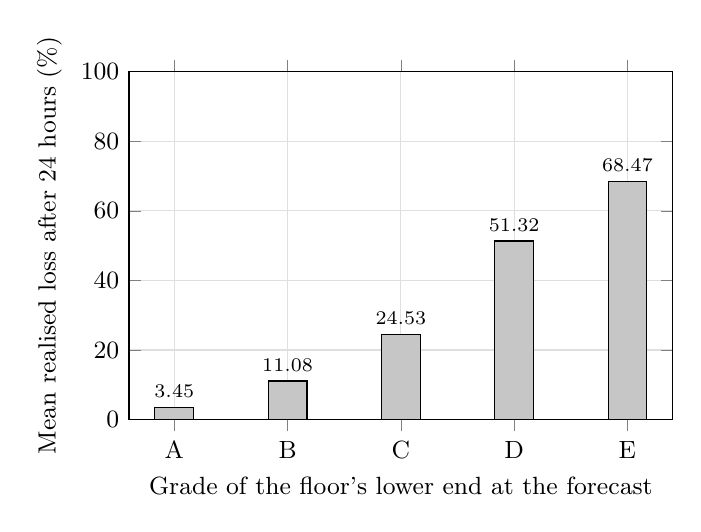
\begin{tikzpicture}
\begin{axis}[ybar, width=0.7\linewidth, height=6cm, bar width=14pt, symbolic x coords={A,B,C,D,E}, xtick=data, xlabel={Grade of the floor's lower end at the forecast}, ylabel={Mean realised loss after 24 hours (\%)}, ymin=0, ymax=100, grid=major, grid style={gray!25}, nodes near coords, nodes near coords style={font=\scriptsize}, tick label style={font=\small}, label style={font=\small}]
\addplot[fill=gray!45] coordinates {(A,3.4511) (B,11.0818) (C,24.5258) (D,51.3220) (E,68.4703)};
\end{axis}
\end{tikzpicture}
\caption{Mean loss of the 100 USDC reference position 24 hours after the forecast, by grade, over rated retrospective records (H4). Records per grade: A: 474; B: 127; C: 80; D: 84; E: 111. Computed by analysis/results.py from the released dataset.}
\label{fig:grades}
\end{figure}


\textbf{Sample-size gates (Section 7.5): not met.} The backfill holds 876 resolved records (the gate is 2,000), launched by 214 distinct creators (an upper bound on creator clusters; the gate is 500), with 127 insider-exit events and no tradability or liquidity events (the gate is 100 per channel). No channel model was fitted. H2, H3 and H6 need one and are not tested; H5 also needs 30 days of wallet history, which no wallet can have before 15 November 2026.

\textbf{Baselines, descriptive only.} Fitting nothing, the comparisons of Section 7.3 can still be run on the insider channel to show the data's shape, but they support no claim. On an out-of-time split with a one-horizon embargo and unseen creators (286 test records, 17 insider exits), B0's Brier score is 0.059 and v1 recalibrated by isotonic regression (B1) scores 0.075, with an AUC of 0.58. The floor's lower end, which is a severity, not a probability, has an AUC of 0.46 for whether an exit occurs. Severity and likelihood are different things, which is the separation Section 5 rests on.

\subsubsection{8.5 Exploratory analyses}\label{exploratory-analyses}

These were not pre-registered and are reported as exploratory.

\emph{H1 measured at the horizon.} The pre-registered event measure compares the position's value just before and at the block in which the event crosses its threshold. When insiders sell gradually, that block carries only the last part of the exit: in the worked example the firing block costs the position 3\% while the whole exit costs it 61\%. Comparing instead the pessimistic insider-exit recovery at the last prior forecast with the recovery at the horizon, for the same 70 launches, the mean absolute difference is 2.8 points (median 0.25); in 16\% of them the horizon value is below the pessimistic floor. The simulated floor predicted where the position ended. The pre-registered criterion is not replaced by this result; it is the evidence that the event measure of Appendix A.5, step 5, should be revised in a later version, with the revision registered before it is tested.

\emph{H4 net of trading costs.} The floor and the realised loss both include the round-trip cost of the reference position, so part of the ordering could be mechanical. Measuring the horizon recovery against each record's own friction removes it. The ordering survives: 0.5\%, 6.0\%, 20.7\%, 49.2\% and 67.5\% from A to E, while mean friction is between 94 and 97 per 100 in every grade.

\subsubsection{8.6 The committed record}\label{the-committed-record}

From its first production record on 8 October 2026 (block 24,825,515) to the dataset's download on 12 October (block 25,607,224), DryDock issued 17,793 records for 4,122 launches and grouped them into 968 batches. Their mix matches the backfill's: 1.6\% rated (the backfill: 1.8\%), 98.4\% too early, 15 unobservable.

None of them counts yet. The committer account that posts roots to the ForecastLedger has not been funded with the USDC Arc charges for gas, so the ledger is not deployed and no root is on chain. Under the rule that a record counts only if its root lands within 1,200 blocks of its forecast block (Appendix A.1, D8), every record issued so far will stay outside the scoreboard even after funding; the batches will still be posted, in order, so that they remain checkable. The pre-registered tests on committed data therefore start from the first record issued after the ledger is live, and the scoreboard is empty until then.

The committed record also exposed an operating limit. Resolving every record with a reference position cost more chain reads per alarm than the free-tier Worker could spend, and by 12 October the live resolver had fallen about 17,000 records behind; it now resolves rated records only, as the backfill does (D14).

\subsection{9. Worked examples}\label{worked-examples}

The first example is a real launch from the backfill, chosen by a fixed rule before its numbers were read: the first rated 1-hour record, by block, whose insider-exit event fired before its horizon and whose floor is an interval. The second is a hypothetical launch that isolates the arithmetic.

\subsubsection{9.1 A real launch}\label{a-real-launch}

TOLLYTOAD (\texttt{0x517b95ae1f8ccafaba3d84eb66e9df007b2ca88a}) was created on Tolly at block 21,087,614, under three hours after mainnet opened, in a Uniswap V3 pool with a 1\% fee and no hook. Its first swap came 69 blocks later. The record at the 1-hour landmark (block 21,094,790) reads:

{\def\LTcaptype{none} % do not increment counter
\begin{longtable}[]{@{}
  >{\raggedright\arraybackslash}p{(\linewidth - 2\tabcolsep) * \real{0.5000}}
  >{\raggedright\arraybackslash}p{(\linewidth - 2\tabcolsep) * \real{0.5000}}@{}}
\toprule\noalign{}
\begin{minipage}[b]{\linewidth}\raggedright
Quantity
\end{minipage} & \begin{minipage}[b]{\linewidth}\raggedright
Value
\end{minipage} \\
\midrule\noalign{}
\endhead
\bottomrule\noalign{}
\endlastfoot
Holders & 75 \\
Lower-bound insider set & 0 holders \\
Pessimistic insider set & 65 holders, whose exit would take 3,294 USDC from the pool \\
Independent entities outside the lower bound & 19 \\
Friction (100 USDC in and out, no event) & 98.0 \\
Recovery after tradability or liquidity event & 98.0 (no privileged role; liquidity locked) \\
Recovery after insider exit, lower bound / pessimistic & 98.0 / 38.8 \\
Structural floor & 38.8 to 98.0 USDC per 100; grade D \\
v1 score (1 October / 7 October rule) & 79 / 80, ``Strong setup'' \\
\end{longtable}
}

No holder showed evidence of acting with the creator, so the lower bound is empty and its exit costs nothing. 65 of the 75 holders could not show independence (Section 8.3), and if they all sold the position would keep 38.8 of its 100 USDC. v1 called the launch a strong setup.

Over the next 24 hours the pessimistic set sold 96\% of its tokens; the insider-exit event fired 111,660 blocks (about 16 hours) after the record. At the horizon the position was worth 39.1 USDC. The floor's lower end had said 38.8.

The example also shows the weakness of the pre-registered event measure (Section 8.5): in the single block where the outflow crossed half of the set's balance, the position lost only 3.3\%, because most of the exit had already happened in smaller sales.

\subsubsection{9.2 An illustrative launch}\label{an-illustrative-launch}

One hypothetical launch scores 76 to 83 under v1 and has a structural floor of 11 to 30 USDC per 100 under v2. The launch is constructed for illustration; it is not a real token.

\begin{itemize}
\tightlist
\item
  The pool behaves as a constant-product pool with 25,000 USDC and 10\% of token supply, at a 1\% fee per swap.
\item
  Liquidity is locked by the launchpad. The token and hook have no privileged roles, and the fee is immutable.
\item
  The creator and two creation-block buyers funded by the creator hold 8\% of supply. This is the lower-bound insider set.
\item
  A further 12\% sits in fresh wallets funded through a bridge. With the 8\%, this is the pessimistic set at 20\%.
\item
  The ten largest holders have 30\%. More than 30 wallets bought in the last hour, the price is rising, tracked wallets are holding, and the creator has a prior launch that reached 100k USD and is not selling.
\end{itemize}

\textbf{Scores.}

{\def\LTcaptype{none} % do not increment counter
\begin{longtable}[]{@{}
  >{\raggedright\arraybackslash}p{(\linewidth - 4\tabcolsep) * \real{0.3333}}
  >{\raggedright\arraybackslash}p{(\linewidth - 4\tabcolsep) * \real{0.3333}}
  >{\raggedright\arraybackslash}p{(\linewidth - 4\tabcolsep) * \real{0.3333}}@{}}
\toprule\noalign{}
\begin{minipage}[b]{\linewidth}\raggedright
Quantity
\end{minipage} & \begin{minipage}[b]{\linewidth}\raggedright
v1
\end{minipage} & \begin{minipage}[b]{\linewidth}\raggedright
v2
\end{minipage} \\
\midrule\noalign{}
\endhead
\bottomrule\noalign{}
\endlastfoot
Headline if 8\% insiders are detected & 82.9, ``Strong setup'' & See below \\
Headline if 20\% insiders are detected & 76.3, ``Strong setup'' & See below \\
Friction: 100 USDC in and out, no event & Not reported & Returns 98.0 \\
Loss given tradability event & Not reported & 2.0\% (friction only) \\
Loss given liquidity event & Not reported & 2.0\% (friction only) \\
Loss given insider exit, lower-bound set & Not reported & 69.7\%; insiders take 11,118 USDC, 44\% of the pool's USDC \\
Loss given insider exit, pessimistic set & Not reported & 89.1\%; insiders take 16,699 USDC, 67\% of the pool's USDC \\
Structural floor & Not reported & 10.9 to 30.3 USDC per 100; grade E \\
\end{longtable}
}

The v1 figures assume linear interpolation between the published endpoints. The v2 figures follow from the pool arithmetic alone and are reproduced in Appendix B.

\textbf{Reading the result.}

The two systems are not contradicting each other on a prediction. v1 makes none. What v2 adds at Stage 0 is a fact the v1 number hides: a group that may be one party can remove most of a buyer's money in one block, and the pool's lock does not prevent it.

Whether that group will exit is a separate question, and only outcome data can answer it. Suppose the tradability and liquidity probabilities are near zero and the insider-exit probability over 24 hours is π. The Integrity Score is then 100(1 − πℓ), which gives the values below. The π values are assumptions chosen to show the arithmetic.

{\def\LTcaptype{none} % do not increment counter
\begin{longtable}[]{@{}
  >{\raggedright\arraybackslash}p{(\linewidth - 4\tabcolsep) * \real{0.3333}}
  >{\raggedright\arraybackslash}p{(\linewidth - 4\tabcolsep) * \real{0.3333}}
  >{\raggedright\arraybackslash}p{(\linewidth - 4\tabcolsep) * \real{0.3333}}@{}}
\toprule\noalign{}
\begin{minipage}[b]{\linewidth}\raggedright
Assumed π for insider exit
\end{minipage} & \begin{minipage}[b]{\linewidth}\raggedright
Score with lower-bound loss
\end{minipage} & \begin{minipage}[b]{\linewidth}\raggedright
Score with pessimistic loss
\end{minipage} \\
\midrule\noalign{}
\endhead
\bottomrule\noalign{}
\endlastfoot
0.10 & 93 & 91 \\
0.30 & 79 & 73 \\
0.60 & 58 & 47 \\
\end{longtable}
}

If Arc data show that insiders in this position rarely exit within a day, the calibrated score will be high and v1's optimism about such launches will have been justified. If they usually exit, it will be low. Either way the number will rest on counted outcomes.

\textbf{What would raise it.}

The creator can raise the floor from 11 to 30 by time-locking the 12\% beyond the horizon, and higher still by locking part of the 8\%. Wash volume, more wallets or a higher price do nothing, and net buying lowers it (Proposition 4). Under v1 as published the reverse holds: no rule credits a lock, and the wash volume earns up to 30 points.

\subsection{10. Verifiability and governance}\label{verifiability-and-governance}

A user should not have to trust the platform's arithmetic or its account of its own accuracy. Both are made checkable.

\subsubsection{10.1 A deterministic specification}\label{a-deterministic-specification}

Every output is a pure function of three inputs: Arc state at a finalized block, a versioned specification, and a versioned registry of hubs, lockers and template contracts. The specification, a reference implementation and the hashes of the parameter and registry files are public. Anyone with an archive node can recompute any score ever shown.

Recomputation also enforces time-consistency. A feature that read state after its block would fail to reproduce from state up to that block.

\subsubsection{10.2 Committed forecasts}\label{committed-forecasts}

At fixed intervals the platform posts one transaction to Arc containing the Merkle root of every forecast record issued in that interval. A record holds the token, the block, the horizon, the version hashes, the three losses, the three probability intervals and the score. The page for any token can supply an inclusion proof for the number it displays.

Resolution at the end of the horizon is a deterministic function of chain state. The scoreboard is therefore a function of two public things: the committed forecasts and the chain. This rules out silent revision, selective reporting and accuracy claims assembled in hindsight. It is pre-registration applied to every forecast, and it parallels the launch certificate of {[}4{]}, which binds a launch's claims before money moves.

A commitment shows that a forecast was made when claimed. It does not show that the forecast was computed correctly. Section 10.1 covers that.

In DryDock's implementation the roots go to a ForecastLedger contract on Arc (Appendix A.4), one transaction every 600 blocks. A record counts as committed only if its root landed within 1,200 blocks of its forecast block; a record posted later is published and resolved like any other but is left out of the scoreboard. The records themselves, their leaves and their resolutions are published by batch, so anyone can recompute every leaf, check every root against the contract, and recompute the scoreboard.

\subsubsection{10.3 Versioning}\label{versioning}

A new model version runs in shadow first. Its forecasts are committed but not displayed until at least 1,000 have resolved. It is promoted only if it passes the ship criteria of Section 7.6 against the incumbent. Past forecasts keep the label of the version that issued them, and each change is logged with its reason.

\subsubsection{10.4 No discretion}\label{no-discretion}

No score is adjusted by hand. Registry entries are the one place where human judgement enters, for example recognising a locker contract or an exchange wallet. Each entry is public, dated and justified, and can be challenged. Errors are corrected in later versions. The committed record is never rewritten.

\subsubsection{10.5 Labels on addresses}\label{labels-on-addresses}

A public label on a wallet is a statement about a person who cannot reply. The risk page already concedes that attribution errs {[}2{]}. Labels should therefore carry their evidence, be phrased as likelihoods, and be withheld below the evidence thresholds of Section 5.8. ``Losing trader'' serves no reader and should be dropped.

\subsection{11. Limitations and non-goals}\label{limitations-and-non-goals}

\textbf{Validation is partial and retrospective.} Section 8 tests the two hypotheses that need no fitted model (H1 and H4) on records recomputed after their outcomes (D1). That v2's probabilities forecast better than v1 remains a hypothesis until a channel model is fitted, which the sample-size gates of Section 7.5 govern; Section 8.4 reports the counts. The committed record began on 8 October 2026.

\textbf{The audit was checked against the code afterwards.} The first version read only the page. Section 3.3 marks each finding against the v1 source; one conclusion (F1) was wrong and one number (F5) was understated.

\textbf{Closed forms are illustrations.} Propositions 1 and 4 and every numerical example assume a constant-product pool. The launchpads use Uniswap V3 and V4 pools {[}3, 53, 54{]}. The same algebra holds wherever liquidity is constant across the price range traversed, as with a single wide position, but magnitudes on real pools must come from simulation.

\textbf{The pessimistic bound is wide on a young chain.} The history margin asks for activity 30 days before a token's creation, and public mainnet opened on 16 September 2026, so for launches before mid-October only addresses active before mainnet opened can pass it. The lower end of the floor can therefore be low for sound launches. The interval is honest about this, and the letter grade may be uninformative until the chain ages (Section 12, objection 2). Section 8.3 measures how wide it is.

\textbf{Public infrastructure bounds the evidence.} The funding lookback is 12 hours, not 7 days (D2), because public Arc nodes keep less history than the design assumed. Funding older than that cannot link wallets, which narrows the lower-bound set; the pessimistic set does not depend on it.

\textbf{Structural risk is not all risk.} A launch with an Integrity Score of 95 can still fall to zero because nobody wants the token. The score measures whether the structure can take a buyer's money, not whether the market will.

\textbf{Off-chain evidence is excluded.} Social activity, team identity and code audits are outside the design. This is deliberate. They cannot be recomputed from chain state (R7).

\textbf{Independence is assumed in the score formula.} Insider exits and liquidity withdrawals may be correlated. The decile check in Section 7.6 detects the resulting error but does not repair it. A joint model is future work.

\textbf{Code analysis is incomplete.} No analyser decides what arbitrary contract code can do. Unknown is scored as unbounded, which penalises honest custom contracts.

\textbf{Forecasts are bounded by their horizon.} Nothing here speaks to day eight.

\textbf{Evidence is borrowed from other chains.} Most cited findings come from Solana, Ethereum and BNB Chain. Their transfer to Arc, with institutional validators, USDC gas and different launchpads, is assumed, not shown.

\textbf{This is not advice, and law is out of scope.} Publishing forecasts about tradable assets may carry obligations in some jurisdictions. As in {[}4{]}, we flag the question and do not resolve it.

\subsection{12. Adversarial self-review}\label{adversarial-self-review}

We put eight objections to the paper that a hostile referee would raise. Two of them change the design.

\textbf{Objection 1. The audit attacks a summary page, not the system.} Accepted and resolved: Section 3.3 checks every finding against the v1 source code. Ten of twelve hold; F1's conclusion was wrong because the code normalised the score, and F11 used a slightly different rule than the page described. The page is still what users were told, so its inaccuracies are findings in their own right.

\textbf{Objection 2. The floor will grade nearly everything E.} Accepted as a real risk, and the design is changed. If more than 80\% of launches on a launchpad share one Stage 0 grade, the letter is replaced on that launchpad by the floor interval and its percentile rank among launches of the same age. The grade distribution is reported monthly. In the first data the risk did not materialise: among rated records, grade A is the most common on Argus (57\%) and Tolly (34\%), and no launchpad has more than 80\% of its rated records in one grade (Section 8.2; Arcora's eight rated records are too few to judge).

\textbf{Objection 3. Dropping demand and momentum discards the best predictors.} Speed of accumulation is the strongest predictor of graduation on Pump.fun {[}10{]}. Graduation is a different estimand from structural failure. Those variables remain visible in the market panel, H6 measures what the score loses, and the paper accepts that loss in exchange for Proposition 4. A product that forecasts upside is a legitimate separate product with a different threat model.

\textbf{Objection 4. The event thresholds are as arbitrary as v1's weights.} The thresholds define what is forecast. They do not decide whether a forecast was right. A different threshold yields a different, equally testable forecast, and Section 7.7 reports whether conclusions depend on the choice. A weight has no such test.

\textbf{Objection 5. Calibration cannot hold against adaptive adversaries.} Accepted in part. Calibration is a property of a window of past forecasts. Adaptive conformal methods bound long-run miscoverage under shift {[}32{]}, and the kill criteria revert the display when calibration breaks. The severity layer does not depend on calibration at all, which is why it ships first.

\textbf{Objection 6. A public specification helps attackers.} It does help the aged-wallet attacker, who learns the history margin. The alternative is a score nobody can check, which fails R7 and R8 and the standard of {[}4{]}. Proposition 5 shows that the other routes to a better score are routes to a safer launch.

\textbf{Objection 7. The independence test will exclude honest newcomers and so penalise fair launches.} Accepted, and the design is changed. The pessimistic set is never shown alone. Every display carries both ends of the interval, and the forecasting layer, not a rule, decides how much the pessimistic end matters once outcomes exist. On Arc's first three weeks the cost is visible: the pessimistic set holds every holder in 63\% of records (Section 8.3).

\textbf{Objection 8. The author both proposes and evaluates.} Accepted. The remedy is structural: forecasts are committed before outcomes, baselines include the strongest version of v1, the data and code are released with this paper (Appendix C), and independent replication is invited. The author also built the implementation, so a defect in it could bias the results in either direction. One did: the first backfill valued held positions against a pool that lacked their own purchase, which made grade A look worst, and it was found and corrected before any result was written (D13). Every record can be recomputed from public chain state with the released code. Citations were checked to the differing degrees stated in the verification note.

\subsection{13. Conclusion and roadmap}\label{conclusion-and-roadmap}

The current score adds things that should not be added, in units that mean nothing, toward a target it does not name. Its most heavily weighted inputs are the ones an insider can buy for a few hundred USDC of fees. None of this is unusual for the category. It is the category's standard, and that is the opportunity.

The replacement rests on one separation. What a launch's structure permits is a fact, computable today from chain state by simulation, with no training data. Whether those who can act will act is a probability, estimable only from outcomes, and publishable only once it is calibrated. Stating the first without waiting for the second gives users a true and useful number now. Committing the second on-chain before it resolves gives them a reason to believe it later.

The design does not solve Sybil identity, and it says so. It bounds what cannot be identified, puts the burden of proof on independence, and enumerates the one remaining route to gaming.

\subsubsection{Implementation order and status}\label{implementation-order-and-status}

\begin{enumerate}
\def\labelenumi{\arabic{enumi}.}
\tightlist
\item
  \textbf{Corrections to v1.} Superseded: DryDock retired v1 entirely on 8 October 2026 instead of correcting it. v1 survives only as the baselines B1 and B2 (Appendix C).
\item
  \textbf{Stage 0.} Done on 8 October 2026: the simulator, the two insider sets, the registry and the abstentions are live, and the floor interval with its losses given event is the headline on every token page. Records are issued at the five landmarks, batched for the ForecastLedger and resolved after 24 hours. \emph{Gate: a third party reproduces a sample of published floors from its own archive node. Open.}
\item
  \textbf{Shadow.} Not started: the sample-size counts of Section 7.5 are not met (876 resolved records, 214 creators, no tradability or liquidity events; Section 8.4), so no channel model is fitted. The scoreboard is live for the committed record.
\item
  \textbf{Stage 1.} Pending. \emph{Gate: H2 and H3.}
\item
  \textbf{Stage 2.} Pending. \emph{Gate: all five ship criteria of Section 7.6.}
\item
  \textbf{External review.} Data and code are released with this version and the paper is posted as a working paper. Replication and red-teaming are invited; peer review is pending.
\end{enumerate}

\subsection{References}\label{references}

{[}1{]} DryDock. How the DryDock score works. Updated 1 October 2026. \href{https://drydockprotocol.org/methodology}{drydockprotocol.org/methodology}

{[}2{]} DryDock. Risk disclosure. Updated 1 October 2026. \href{https://drydockprotocol.org/risk}{drydockprotocol.org/risk}

{[}3{]} DryDock. Launchpads. \href{https://drydockprotocol.org/launchpads}{drydockprotocol.org/launchpads}

{[}4{]} F. Ghasemlu. The Verifiable Launch: A Trust-Minimized Protocol for Audit-Gated Token Deployment. Draft of July 2026. \href{https://drydockprotocol.org/research/verifiable-launch}{drydockprotocol.org/research/verifiable-launch}

{[}5{]} P. Xia, H. Wang, B. Gao, W. Su, Z. Yu, X. Luo, C. Zhang, X. Xiao, G. Xu. Trade or Trick? Detecting and Characterizing Scam Tokens on Uniswap Decentralized Exchange. Proc. ACM Meas. Anal. Comput. Syst. 5(3), article 39, 2021. \href{https://doi.org/10.1145/3491051}{doi:10.1145/3491051}

{[}6{]} B. Mazorra, V. Adan, V. Daza. Do Not Rug on Me: Leveraging Machine Learning Techniques for Automated Scam Detection. Mathematics 10(6):949, 2022. \href{https://arxiv.org/abs/2201.07220}{arXiv:2201.07220}

{[}7{]} F. Cernera, M. La Morgia, A. Mei, F. Sassi. Token Spammers, Rug Pulls, and Sniper Bots: An Analysis of the Ecosystem of Tokens in Ethereum and in the Binance Smart Chain (BNB). USENIX Security 2023. \href{https://www.usenix.org/conference/usenixsecurity23/presentation/cernera}{usenix.org}

{[}8{]} D. Sun, W. Ma, L. Nie, Y. Liu. SoK: Comprehensive Analysis of Rug Pull Causes, Datasets, and Detection Tools in DeFi. 2024. \href{https://arxiv.org/abs/2403.16082}{arXiv:2403.16082}

{[}9{]} M. Naviglio, F. Tarantelli, F. Lillo. Price manipulation schemes of new crypto-tokens in decentralized exchanges. 2025. \href{https://arxiv.org/abs/2502.10512}{arXiv:2502.10512}

{[}10{]} G. Marino, M. Naviglio, F. Tarantelli, F. Lillo. Predicting the success of new crypto-tokens: the Pump.fun case. 2026. \href{https://arxiv.org/abs/2602.14860}{arXiv:2602.14860}

{[}11{]} W. Ding, Y. Luo, J. Xu. Decompose Market Manipulation Strategies: Evidence from On-chain Meme Coin Market. Working paper, Sydney Banking and Financial Stability Conference, 2025. \href{https://sbfc.sydney.edu.au/2025/papers/SBFC2025_4G3_P154.pdf}{sbfc.sydney.edu.au}. Later version with C. Lin as an additional author: SSRN 5953738. \href{https://papers.ssrn.com/abstract=5953738}{papers.ssrn.com}

{[}12{]} Y. Luo, Y. Feng, J. Xu, Y. Liu. Resisting Manipulative Bots in Meme Coin Copy Trading: A Multi-Agent Approach with Chain-of-Thought Reasoning. 2026. \href{https://arxiv.org/abs/2601.08641}{arXiv:2601.08641}

{[}13{]} A. M. Mongardini, A. Mei. A Midsummer Meme's Dream: Investigating Market Manipulations in the Meme Coin Ecosystem. 2025, revised 2026. \href{https://arxiv.org/abs/2507.01963}{arXiv:2507.01963}

{[}14{]} Solidus Labs. The 2025 Rug Pull Report: Rug Pulls and Pump-and-Dumps on Solana. May 2025. \href{https://www.soliduslabs.com/reports/solana-rug-pulls-pump-dumps-crypto-compliance}{soliduslabs.com}. Reported by L. Jakobson, ``Alarming'' 99\% of Memecoin Launches on PumpFun are Pump-and-Dumps or Rug Pulls: Report, The Defiant, 9 May 2025. \href{https://thedefiant.io/news/defi/alarming-99-of-memecoin-launches-on-pumpfun-are-pump-and-dumps-or-rug-pulls-report}{thedefiant.io}

{[}15{]} Pine Analytics. Exit Liquidity Machines: Dissecting Pump.fun Farming. 21 April 2025. \href{https://pineanalytics.substack.com/p/exit-liquidity-machines}{pineanalytics.substack.com}

{[}16{]} F. Victor, A. M. Weintraud. Detecting and Quantifying Wash Trading on Decentralized Cryptocurrency Exchanges. The Web Conference 2021, 23--32. \href{https://doi.org/10.1145/3442381.3449824}{doi:10.1145/3442381.3449824}

{[}17{]} L. W. Cong, X. Li, K. Tang, Y. Yang. Crypto Wash Trading. Management Science 69(11):6427--6454, 2023. \href{https://doi.org/10.1287/mnsc.2021.02709}{doi:10.1287/mnsc.2021.02709}

{[}18{]} C. F. Torres, M. Steichen, R. State. The Art of the Scam: Demystifying Honeypots in Ethereum Smart Contracts. USENIX Security 2019.

{[}19{]} S. Meiklejohn, M. Pomarole, G. Jordan, K. Levchenko, D. McCoy, G. M. Voelker, S. Savage. A Fistful of Bitcoins: Characterizing Payments Among Men with No Names. ACM Internet Measurement Conference 2013, 127--140.

{[}20{]} F. Victor. Address Clustering Heuristics for Ethereum. Financial Cryptography and Data Security 2020, Lecture Notes in Computer Science, 617--633. \href{https://doi.org/10.1007/978-3-030-51280-4_33}{doi:10.1007/978-3-030-51280-4\_33}

{[}21{]} J. R. Douceur. The Sybil Attack. International Workshop on Peer-to-Peer Systems (IPTPS) 2002, Lecture Notes in Computer Science 2429, 251--260.

{[}22{]} C. F. Manski. Partial Identification of Probability Distributions. Springer, 2003.

{[}23{]} G. W. Brier. Verification of forecasts expressed in terms of probability. Monthly Weather Review 78(1):1--3, 1950.

{[}24{]} A. H. Murphy. A new vector partition of the probability score. Journal of Applied Meteorology 12(4):595--600, 1973. \href{https://doi.org/10.1175/1520-0450(1973)012\%3C0595:ANVPOT\%3E2.0.CO;2}{doi:10.1175/1520-0450(1973)012\textless0595:ANVPOT\textgreater2.0.CO;2}

{[}25{]} T. Gneiting, A. E. Raftery. Strictly proper scoring rules, prediction, and estimation. Journal of the American Statistical Association 102(477):359--378, 2007.

{[}26{]} J. C. Platt. Probabilistic outputs for support vector machines and comparisons to regularized likelihood methods. In Advances in Large Margin Classifiers, MIT Press, 2000, 61--74 (chapter listed by the publisher as ``Probabilities for SV Machines'').

{[}27{]} B. Zadrozny, C. Elkan. Transforming classifier scores into accurate multiclass probability estimates. ACM SIGKDD 2002, 694--699.

{[}28{]} A. Niculescu-Mizil, R. Caruana. Predicting good probabilities with supervised learning. ICML 2005, 625--632.

{[}29{]} B. Van Calster, D. J. McLernon, M. van Smeden, L. Wynants, E. W. Steyerberg. Calibration: the Achilles heel of predictive analytics. BMC Medicine 17:230, 2019.

{[}30{]} E. W. Steyerberg et al.~Assessing the performance of prediction models: a framework for traditional and novel measures. Epidemiology 21(1):128--138, 2010.

{[}31{]} V. Vovk, I. Petej. Venn-Abers predictors. Uncertainty in Artificial Intelligence 2014. \href{https://arxiv.org/abs/1211.0025}{arXiv:1211.0025}

{[}32{]} I. Gibbs, E. Candès. Adaptive conformal inference under distribution shift. Advances in Neural Information Processing Systems 34 (NeurIPS 2021), 1660--1672.

{[}33{]} M. Hardt, N. Megiddo, C. Papadimitriou, M. Wootters. Strategic classification. Innovations in Theoretical Computer Science 2016, 111--122.

{[}34{]} J. Kleinberg, M. Raghavan. How do classifiers induce agents to invest effort strategically? ACM Transactions on Economics and Computation 8(4), article 19, 2020. \href{https://doi.org/10.1145/3417742}{doi:10.1145/3417742}. Conference version: ACM EC 2019, 825--844; \href{https://arxiv.org/abs/1807.05307}{arXiv:1807.05307}.

{[}35{]} J. C. Perdomo, T. Zrnic, C. Mendler-Dünner, M. Hardt. Performative prediction. ICML 2020.

{[}36{]} C. A. E. Goodhart. Problems of monetary management: the U.K. experience. Papers in Monetary Economics, Reserve Bank of Australia, 1975. Reprinted in Monetary Theory and Practice, Macmillan, 1984, 91--121.

{[}37{]} M. Nardo, M. Saisana, A. Saltelli, S. Tarantola, A. Hoffmann, E. Giovannini. Handbook on Constructing Composite Indicators: Methodology and User Guide. OECD, 2008.

{[}38{]} R. M. Dawes. The robust beauty of improper linear models in decision making. American Psychologist 34(7):571--582, 1979.

{[}39{]} L. Barras, O. Scaillet, R. Wermers. False discoveries in mutual fund performance: measuring luck in estimated alphas. Journal of Finance 65(1):179--216, 2010.

{[}40{]} E. F. Fama, K. R. French. Luck versus skill in the cross-section of mutual fund returns. Journal of Finance 65(5):1915--1947, 2010.

{[}41{]} Y. Benjamini, Y. Hochberg. Controlling the false discovery rate: a practical and powerful approach to multiple testing. Journal of the Royal Statistical Society B 57(1):289--300, 1995.

{[}42{]} B. Efron, C. Morris. Data analysis using Stein's estimator and its generalizations. Journal of the American Statistical Association 70(350):311--319, 1975.

{[}43{]} D. R. Cox. Regression models and life-tables. Journal of the Royal Statistical Society B 34(2):187--202, 1972.

{[}44{]} H. C. van Houwelingen. Dynamic prediction by landmarking in event history analysis. Scandinavian Journal of Statistics 34(1):70--85, 2007.

{[}45{]} M. López de Prado. Advances in Financial Machine Learning. Wiley, 2018.

{[}46{]} F. X. Diebold, R. S. Mariano. Comparing predictive accuracy. Journal of Business and Economic Statistics 13(3):253--263, 1995.

{[}47{]} J. A. Hanley, B. J. McNeil. The meaning and use of the area under a receiver operating characteristic (ROC) curve. Radiology 143(1):29--36, 1982.

{[}48{]} T. Saito, M. Rehmsmeier. The precision-recall plot is more informative than the ROC plot when evaluating binary classifiers on imbalanced datasets. PLoS ONE 10(3):e0118432, 2015.

{[}49{]} A. J. Vickers, E. B. Elkin. Decision curve analysis: a novel method for evaluating prediction models. Medical Decision Making 26(6):565--574, 2006.

{[}50{]} G. S. Collins, J. B. Reitsma, D. G. Altman, K. G. M. Moons. Transparent reporting of a multivariable prediction model for individual prognosis or diagnosis (TRIPOD). Annals of Internal Medicine 162(1):55--63, 2015.

{[}51{]} G. Gigerenzer, U. Hoffrage. How to improve Bayesian reasoning without instruction: frequency formats. Psychological Review 102(4):684--704, 1995.

{[}52{]} P. Bolton, X. Freixas, J. Shapiro. The credit ratings game. Journal of Finance 67(1):85--111, 2012. \href{https://doi.org/10.1111/j.1540-6261.2011.01708.x}{doi:10.1111/j.1540-6261.2011.01708.x}

{[}53{]} H. Adams, N. Zinsmeister, M. Salem, R. Keefer, D. Robinson. Uniswap v3 Core. Whitepaper, March 2021. \href{https://uniswap.org/whitepaper-v3.pdf}{uniswap.org/whitepaper-v3.pdf}

{[}54{]} H. Adams, M. Salem, N. Zinsmeister, S. Reynolds, A. Adams, W. Pote, M. Toda, A. Henshaw, E. Williams, D. Robinson. Uniswap v4 Core. Whitepaper, August 2024. \href{https://uniswap.org/whitepaper-v4.pdf}{uniswap.org/whitepaper-v4.pdf}

{[}55{]} G. Angeris, T. Chitra. Improved price oracles: constant function market makers. ACM Advances in Financial Technologies 2020.

{[}56{]} M. O. Hill. Diversity and evenness: a unifying notation and its consequences. Ecology 54(2):427--432, 1973.

{[}57{]} Arc network facts (mainnet date, USDC gas, block time, finality, opt-in privacy): \href{https://stablecoininsider.org/arc-mainnet-live/}{Stablecoin Insider, ``Arc Mainnet Is Live''}; \href{https://coin360.com/news/circle-arc-mainnet-launch-revenue-miss}{Coin360, ``Circle Sets September 16 Launch for Arc Mainnet''}; \href{https://decrypt.co/340212/what-is-arc-the-stablecoin-blockchain-from-usdc-issuer-circle}{Decrypt, ``What Is Arc?''}

{[}58{]} Existing scores: \href{https://www.dextools.io/tutorials/what-is-dext-score-token-audit}{DEXTools, ``What Is the DEXT Score? How to Read DEXTools Token Audits''}; \href{https://docs.solanatracker.io/guides/token-safety.md}{Solana Tracker, ``Token Safety and Rugcheck''}

{[}59{]} Blockworks. Are 97\% of Tokens on Uniswap Really Rug Pulls? 2 November 2022. \href{https://blockworks.com/news/are-97-of-tokens-on-uniswap-really-rug-pulls}{blockworks.com}

{[}60{]} A. Gelman, J. Hill. Data Analysis Using Regression and Multilevel/Hierarchical Models. Cambridge University Press, 2007 (published December 2006).

\subsubsection{Verification note}\label{verification-note}

Every reference was checked on 7 October 2026, and the checks the first version listed as open were completed on 8 October 2026, to the differing degrees listed below. A reader should weigh them accordingly.

\begin{itemize}
\tightlist
\item
  \textbf{Full text fetched and read:} {[}1{]} to {[}4{]}, {[}6{]} (the labelling method, Section 6 of the arXiv version), {[}10{]}, {[}11{]} (the conference version), {[}12{]}, {[}14{]} (the Solidus Labs report's web page), {[}53{]}, {[}54{]}.
\item
  \textbf{Abstract, article or publisher page fetched and read:} {[}5{]}, {[}7{]} to {[}9{]}, {[}13{]}, {[}15{]}, {[}16{]}, {[}18{]}, {[}31{]}, {[}35{]}, {[}55{]}, {[}59{]}, the Stablecoin Insider item of {[}57{]}, the Solana Tracker item of {[}58{]}, and the SSRN listing of {[}11{]}.
\item
  \textbf{Bibliographic details matched against a Crossref record (volume, issue and pages as deposited by the publisher):} {[}17{]}, {[}19{]}, {[}21{]}, {[}24{]}, {[}25{]}, {[}26{]}, {[}27{]}, {[}28{]}, {[}29{]}, {[}30{]}, {[}33{]}, {[}34{]}, {[}36{]} (the 1984 reprint), {[}37{]}, {[}38{]}, {[}41{]}, {[}42{]}, {[}43{]}, {[}47{]}, {[}50{]}, {[}51{]}, {[}52{]}, {[}56{]}, {[}60{]}. Matched against a Crossref or RePEc record in the first round of checks: {[}20{]}, {[}22{]}, {[}23{]}, {[}39{]}, {[}40{]}, {[}44{]}, {[}46{]}, {[}48{]}, {[}49{]}.
\item
  \textbf{Matched against the proceedings publisher's own record:} {[}32{]} (NeurIPS proceedings, volume 34, pages 1660 to 1672).
\item
  \textbf{Existence, authors, title and venue confirmed by search only:} {[}45{]} (a book, cited without pages) and the DEXTools item of {[}58{]}, whose page appears in search results with the description quoted in Section 2.7 but returned HTTP 404 to a direct request on 8 October 2026.
\item
  \textbf{Read only as search excerpts:} the Coin360 and Decrypt items of {[}57{]}.
\end{itemize}

The completed checks changed six details. {[}24{]} is confirmed. {[}34{]} has a journal version, ACM Transactions on Economics and Computation 8(4), 2020. {[}43{]} runs to page 202; the first version's 220 included the published discussion. {[}26{]} appeared in 2000 at pages 61 to 74, under the chapter title ``Probabilities for SV Machines''. {[}14{]} now cites the Solidus Labs report itself, which gives 98.6\% for Pump.fun tokens with at least five trades. {[}52{]}: the first version had 85 to 111 and its verification note changed this to 85 to 112 from RePEc; the publisher's Crossref deposit gives 85 to 111, which is restored (the publisher's page refused automated requests). Lookups through OpenAlex, Europe PMC and PubMed were not needed.

Two cautions still apply. {[}14{]} is an industry report whose method is described only on its web page. {[}11{]} is a working paper whose author list differs between versions: the conference paper cited here lists Ding, Luo and Xu; the later SSRN version adds Chen Lin.

\subsection{Appendix A. Normative specification}\label{appendix-a.-normative-specification}

This appendix fixes the definitions an implementer needs. Where it conflicts with the body, the appendix governs. Every default is subject to the sensitivity analyses of Section 7.7. This is version 2.0.3, the specification DryDock runs; entries marked † changed from the first version of the paper, for the reasons given in Section 7.8. Its keccak-256 hash enters every record as \texttt{spec\_hash}.

\subsubsection{A.1 Constants and defaults}\label{a.1-constants-and-defaults}

{\def\LTcaptype{none} % do not increment counter
\begin{longtable}[]{@{}
  >{\raggedright\arraybackslash}p{(\linewidth - 4\tabcolsep) * \real{0.3333}}
  >{\raggedright\arraybackslash}p{(\linewidth - 4\tabcolsep) * \real{0.3333}}
  >{\raggedright\arraybackslash}p{(\linewidth - 4\tabcolsep) * \real{0.3333}}@{}}
\toprule\noalign{}
\begin{minipage}[b]{\linewidth}\raggedright
Symbol
\end{minipage} & \begin{minipage}[b]{\linewidth}\raggedright
Meaning
\end{minipage} & \begin{minipage}[b]{\linewidth}\raggedright
Default
\end{minipage} \\
\midrule\noalign{}
\endhead
\bottomrule\noalign{}
\endlastfoot
B & Reference notional & 100 USDC; 1,000 USDC for the depth line \\
H & Horizons & 24 hours primary; 1 hour and 7 days secondary \\
Landmarks & Token ages after the first swap at which forecasts are issued and evaluated & 1 min, 10 min, 1 h, 6 h, 24 h; the forecast block is the first block whose timestamp reaches the landmark \\
δ\_T & Recovery drop that defines a tradability event & 20 points \\
λ\_L & Share of quote-side liquidity withdrawn that defines a liquidity event & 50\% \\
σ\_I & Share of the pessimistic set's tokens net-sold that defines an insider exit & 50\% \\
Severe loss & All-cause endpoint for the market panel & Reference position returns 20 USDC or less at the horizon \\
W & Launch window for the independence test & 20 blocks, about 10 seconds, as in v1 {[}1{]} \\
d & Funding-path depth for the lower-bound set & 3 hops \\
Funding lookback † & Window before a wallet's first purchase that every edge of its funding path must fall in & 86,400 blocks, about 12 hours \\
Materiality † & A transfer links two wallets only if it carried at least this share of what the recipient then spent (its first purchase) or forwarded (the next edge on the path) & 50\% \\
History margin & Minimum address history for independence: transactions sent (nonce) at least 1 at the block 30 days before token creation and at least 10 at the block before creation & 30 days and 10 transactions \\
Dust & Transfers below this never create a link & 1 USDC \\
Minimum evidence † & Below this the state is ``too early'' & 60 seconds of block time since creation, and 10 entities outside the lower-bound set \\
Interval width & Above this the state is ``low confidence'' & 0.40 \\
Commit interval & Blocks between Merkle-root postings & 600 blocks, about 5 minutes \\
Commitment deadline † & A record counts as committed only if its root was posted within this many blocks of its forecast block & 1,200 blocks \\
Individual sellers † & Insiders sold one by one in the exit simulation; the rest of a larger set is sold as one block & 100 \\
Shadow length & Resolved forecasts before a version can be promoted & 1,000 \\
\end{longtable}
}

\subsubsection{A.2 Simulation of losses}\label{a.2-simulation-of-losses}

\begin{enumerate}
\def\labelenumi{\arabic{enumi}.}
\tightlist
\item
  Take Arc state at finalized block \emph{h}. Each scenario is a separate \texttt{eth\_call} at \emph{h} (or several scenarios in one call, each isolated in a reverting sub-call), so every scenario starts from the same state.
\item
  Place the simulator's runtime code, by state override, at a fresh address and at every address that acts in the scenario. Code placed at an address acts as that address: the pool, its hook, the position managers and the token apply their own rules to the real owner.
\item
  From the fresh address, buy \emph{B} USDC of the token through its main pool. Record the tokens received, \emph{q}.
\item
  \textbf{Friction.} Sell \emph{q}. Record the USDC returned.
\item
  \textbf{Tradability.} For each privileged role in the registry, act as its holder and set each parameter to the worst value the code allows without a timelock longer than \emph{H}. Sell \emph{q}, record. If the token or the hook is not a registered template, record zero, set the flag ``unbounded'' and the state ``unobservable''. A scenario with no step returns the friction result.
\item
  \textbf{Liquidity.} For each position whose owner is neither burned nor a recognised lock (registry), act as the owner and withdraw it: \texttt{decreaseLiquidity} and \texttt{collect} for a V3 position NFT, \texttt{modifyLiquidities} for a V4 position NFT, \texttt{burn} and \texttt{collect} or a PoolManager unlock for a direct position. Sell \emph{q}, record.
\item
  \textbf{Insider exit.} For each address in the insider set, in descending order of balance, sell its full balance through the pool. Beyond the first 100 addresses, credit the remaining balance to one further seller by a storage override of the token's balance mapping and sell it in one block. Sell \emph{q}, record. Run once for the lower-bound set and once for the pessimistic set.
\item
  A reverted sale records zero; a reverted event step is recorded as not taken. Each loss given event is 1 minus the recorded amount divided by \emph{B}. If the purchase in step 3 reverts, the state is ``unobservable''.
\end{enumerate}

\subsubsection{A.3 Entity resolution}\label{a.3-entity-resolution}

\begin{enumerate}
\def\labelenumi{\arabic{enumi}.}
\tightlist
\item
  \textbf{Activity.} From the token's transfers up to \emph{h}: in a transaction with a transfer out of the market (the V3 pool or the V4 PoolManager), wallets whose balance rose purchased; in one with a transfer into the market, wallets whose balance fell sold; any other rise is an off-market receipt, credited to the transaction's largest sender. Registry hubs, lockers, the hook, the token and burn addresses are infrastructure, not wallets.
\item
  \textbf{Seeds.} The creator, wallets that purchased in the launch block, and recipients of off-market receipts from the creator or a launchpad contract before their first purchase.
\item
  \textbf{Links.} Funding: a USDC transfer of at least 1 USDC from a non-hub sender, inside the recipient's lookback window, carrying at least half of what the recipient then spent or forwarded, traced back up to \emph{d} hops; the wallet is linked to every ancestor. A path is traced only into accounts without contract code (an EIP-7702 delegation counts as an account): a transfer from a contract links the recipient to the contract, but the contract's own inflows are not followed. Receipts: an off-market receipt before a first purchase links recipient and sender. Proceeds: a USDC transfer of at least 1 USDC to a non-hub address, after a sale, carrying at least half of the sale proceeds so far, links seller and recipient.
\item
  \textbf{Lower-bound set.} Holders at \emph{h} in a component of the link graph that contains a seed.
\item
  \textbf{Pessimistic set.} The lower-bound set plus every holder that fails any of: the history margin; a first purchase more than \emph{W} blocks after the launch block; funding that is not only from fresh unlabelled addresses (at least one direct funder is a hub or passes the history margin, or there is no direct funder).
\item
  \textbf{Entities.} Purchasers outside the lower-bound set, grouped by component of the link graph.
\end{enumerate}

\subsubsection{A.4 Forecast record and commitment}\label{a.4-forecast-record-and-commitment}

\begin{verbatim}
record = {
  token, pool, block_h, landmark, horizon,
  spec_hash, params_hash, registry_hash,
  friction, loss_T, loss_L, loss_I_lower, loss_I_pessimistic,
  floor_low, floor_high,
  pi_T: [low, high], pi_L: [low, high], pi_I: [low, high],
  score: [low, high],
  state,           // rated | too_early | unobservable | low_confidence
  model            // version of the model that issued the probabilities; zero at Stage 0
}
leaf = keccak256(keccak256(abi.encode(record)))
root = merkle_root(all leaves issued since the last root)   // sorted pairs; posted to the ForecastLedger on Arc
\end{verbatim}

Fractions and probabilities are encoded as parts per million and USDC per 100 as micro-USDC per 100, in fixed-width unsigned integers; \texttt{0xffffffff} encodes null. At Stage 0 the probability and score fields are null, and the losses and floors are null unless the state is ``rated''. The same schema is used at every stage, so the committed history is continuous across upgrades. The ForecastLedger (\texttt{0xC63FA005E73bED90443A1Ffc9e363f573F04Cf23}) stores each root with the block range of its records and the block in which it was posted; it accepts roots only from the committer and can be enumerated with \texttt{count()} and \texttt{commitment(i)}.

\subsubsection{A.5 Resolution}\label{a.5-resolution}

\begin{enumerate}
\def\labelenumi{\arabic{enumi}.}
\tightlist
\item
  For each record, take the first block \emph{e} whose timestamp is at least that of \emph{h} plus \emph{H}.
\item
  Insider exit fires at the first transfer in (\emph{h}, \emph{e}{]} at which the pessimistic set's tokens sent to the market or to addresses outside the set, less tokens bought from the market, reach σ\_I of its balance at \emph{h}.
\item
  Liquidity fires at the first removal in (\emph{h}, \emph{e}{]} at which the quote-side amounts removed by position owners reach λ\_L of the quote-side liquidity at \emph{h} (the V3 pool's USDC balance, or the USDC held by the V4 positions at the pool price).
\item
  Tradability fires if the reference position cannot be bought and sold at \emph{e} while the pool still holds quote liquidity (for V4, the USDC held by the pool's positions at \emph{e}), or if a privileged state change in (\emph{h}, \emph{e}{]} lowers the simulated recovery by δ\_T points. No registered template has such a privilege, so only the first route applies to registered templates.
\item
  The reference position bought at \emph{h} is valued at a later block by buying the same number of tokens there by exact output and selling them straight back: with the pool's liquidity unchanged, the pool as it would stand had the purchase at \emph{h} happened is the pool at that block plus the purchase. For each event that fired, value the position at the block before and at the firing block. Their ratio, times 100, is the realised structural recovery.
\item
  Value the reference position at \emph{e}. Record severe loss if it returns 20 USDC or less.
\item
  Publish the resolution with the record. The scoreboard aggregates only records committed within the deadline.
\end{enumerate}

\subsubsection{A.6 Reporting checklist}\label{a.6-reporting-checklist}

Each scoreboard release states: the specification and registry versions; the date range and count of resolved forecasts by launchpad and landmark; event counts by channel; Brier and logarithmic scores with Murphy components; calibration slope and intercept; reliability diagrams; ROC and precision-recall areas; interval coverage; abstention rate by reason; grade distribution by launchpad; and every comparison against B0 and B1 with its interval.

\subsection{Appendix B. Reproducibility}\label{appendix-b.-reproducibility}

The script below reproduces every number in the paper that is computed rather than measured. It needs Python 3 with numpy and scipy and reads no data. It is \texttt{appendix\_b.py} in the paper's repository, and its output is kept beside it as \texttt{analysis/output/appendix\_b.txt}. The empirical numbers of Section 8 come from \texttt{analysis/results.py} and the released dataset (Appendix C).

\begin{verbatim}
# Reproduces every number computed in the paper other than the empirical results of Section 8, which
# come from analysis/ and the released dataset. Requires Python 3 with numpy and scipy; reads no data.
import numpy as np
from scipy import stats

# --- Section 3, F1 and F3: v1 weights as published, and the normalisation the implementation applied
w = dict(insider=15, top10=10, creator=10, liquidity=15, demand=20, momentum=10, smart=10)
tot = sum(w.values())
print('F1 sum of published weights:', tot)
print('F1 share of attainable needed for the top band if the score were a plain sum: %.1f%%' % (100 * 70 / tot))
# The code (DryDock v1, 1 October 2026) scored points over the points attainable, scaled to 100. Smart money
# counted only when wallet records had loaded, so the attainable total was 80 or 90; on 7 October a
# trading-costs factor (5) was added, giving 85 or 95.
for label, attainable, activity in (('1 Oct, no wallet records', 80, 30), ('1 Oct, wallet records', 90, 40),
                                    ('7 Oct, no wallet records', 85, 30), ('7 Oct, wallet records', 95, 40)):
    print('F1 %s: attainable %d, top band needs 70%% of it; F3 activity share %.1f%%' % (label, attainable, 100 * activity / attainable))

# --- Section 3, F5 and Section 9: the worked example under v1's real rule
def scale(v, bad, good):
    return min(1, max(0, (v - bad) / (good - bad)))
def v1_points(insider, top10, version):
    # Linear between endpoints (verified in the code); holders >= 25 so the 7 October breadth discount is 1.
    p = 15 * scale(insider, .30, .03) + 10 * scale(top10, .50, .15)
    p += 10                                   # creator: an earlier launch reached $100k
    p += 10 * scale(np.log10(25000), np.log10(500), np.log10(25000)) + 5   # depth 25k USDC; custody held by the launchpad
    p += 10 + 5 + 5                           # buyers >= 30, buy pressure >= 65%, organic volume
    p += 10                                   # momentum at full marks
    p += 10                                   # smart money: three winning wallets holding, no snipers
    attainable = 90
    if version == '7 Oct':
        p += 5                                # trading costs: 1% pool fee each way plus the 0.5% swap fee, under 3%
        attainable = 95
    return p, attainable
for version in ('1 Oct', '7 Oct'):
    for ins in (0.08, 0.20):
        p, a = v1_points(ins, .30, version)
        print('F5 v1 (%s) with measured insider share %.0f%%: %.2f of %d points, score %d' % (version, 100 * ins, p, a, round(100 * p / a)))
# F7: the cliff at the 30% insider cap (1 October code, wallet records loaded)
for ins in (0.299, 0.301):
    p, a = v1_points(ins, .30, '1 Oct')
    print('F7 insider share %.1f%%: score %d' % (100 * ins, 30 if ins > .30 else round(100 * p / a)))
# What the first version of the paper computed by assuming a plain sum of the published weights:
lin = lambda v, full, zero, pts: pts * min(1, max(0, (zero - v) / (zero - full)))
for ins in (0.08, 0.20):
    print('F5 plain-sum reading of the published page, insider share %.0f%%: %.1f'
          % (100 * ins, lin(ins, .03, .30, 15) + lin(.30, .15, .50, 10) + 10 + 15 + 20 + 10 + 10))

# --- Section 3, F6 (Proposition 1): constant-product exit impact
for g in (.10, .20, .40):
    for f in (.15, .20, .30):
        print('P1 g=%.2f f=%.2f price drop %.0f%%, quote drained %.0f%%'
              % (g, f, 100 * (1 - (g / (g + f)) ** 2), 100 * f / (g + f)))
    print('P1 g=%.2f insider share giving an 80%% drop: %.1f%%' % (g, 100 * g * (1 / np.sqrt(.2) - 1)))

# --- Section 3, F11: v1's "profitable trader" label under a no-skill null. The code required at least 55%
# of launches won (P&L marked to the current price) and more than $10 ahead; the page said "more than half".
ns = (5, 10, 15, 20, 30, 40, 50)
for q in (.30, .35, .40):
    print('F11 page rule q=%.2f' % q, ['n=%d: %.3f' % (n, stats.binom.sf(n // 2, n, q)) for n in ns])
    print('F11 code rule q=%.2f' % q, ['n=%d: %.3f' % (n, stats.binom.sf(int(np.ceil(.55 * n)) - 1, n, q)) for n in ns])

# --- Section 5.8: shrinkage rule, Beta prior mean .35 weight 20, label iff P(q > .40 | data) > .95
q0, m = .35, 20
for n in ns:
    k = np.arange(n + 1)
    ok = k[stats.beta.sf(q0 + .05, q0 * m + k, (1 - q0) * m + n - k) > .95]
    if len(ok) == 0:
        print('S5.8 n=%d: cannot qualify' % n)
        continue
    kmin = ok.min()
    print('S5.8 n=%d: needs %d wins; false positive %.4f; power at q=.60 %.3f'
          % (n, kmin, stats.binom.sf(kmin - 1, n, q0), stats.binom.sf(kmin - 1, n, .6)))

# --- Section 9.2: v2 facts for the stylised example (constant product, fee retained in the pool)
x0, g, phi, B, S = 25000.0, 0.10, 0.01, 100.0, 1e9
def buy(x, y, usd):
    a = usd * (1 - phi); out = y * a / (x + a); return out, x + usd, y - out
def sell(x, y, tok):
    a = tok * (1 - phi); out = x * a / (y + a); return out, x - out, y + tok
q, x1, y1 = buy(x0, g * S, B)
print('S8 friction: 100 USDC returns %.1f' % sell(x1, y1, q)[0])
for name, f in (('lower-bound set, 8%', .08), ('pessimistic set, 20%', .20)):
    got, x2, y2 = sell(x1, y1, f * S)
    r = sell(x2, y2, q)[0]
    print('S8 insider exit as one block, %s: insiders take %.0f USDC (%.0f%% of pool); reference returns %.1f; loss %.1f%%'
          % (name, got, 100 * got / x1, r, 100 - r))
    for pi in (.10, .30, .60):
        print('   assumed pi=%.2f -> Integrity Score %.0f' % (pi, 100 * (1 - pi * (1 - r / 100))))
# Appendix A.2 sells address by address, largest first. With the split of Section 9.2 (creator 4%, two
# launch-block buyers 2% each; six fresh wallets 2% each) and fees retained in the pool:
for name, parts in (('lower-bound set', [.04, .02, .02]), ('pessimistic set', [.04, .02, .02] + [.02] * 6)):
    x, y = x1, y1
    for f in sorted(parts, reverse=True):
        _, x, y = sell(x, y, f * S)
    print('S8 insider exit address by address, %s: reference returns %.2f' % (name, sell(x, y, q)[0]))
# Uniswap V3 and V4 keep fees outside active liquidity; with fees outside the pool the same example gives:
def sell_ext(x, y, tok):
    a = tok * (1 - phi); out = x * a / (y + a); return out, x - out, y + a
def buy_ext(x, y, usd):
    a = usd * (1 - phi); out = y * a / (x + a); return out, x + a, y - out
q2, xa, ya = buy_ext(x0, g * S, B)
print('S8 fees outside the pool: friction %.1f' % sell_ext(xa, ya, q2)[0])
for f in (.08, .20):
    _, xb, yb = sell_ext(xa, ya, f * S)
    print('S8 fees outside the pool, exit of %.0f%%: reference returns %.1f' % (100 * f, sell_ext(xb, yb, q2)[0]))

# --- Section 7.5: sample sizes
z = stats.norm.ppf(.975)
for p in (.5, .9):
    print('S7.5 bin rate %.1f to within 5 points: n=%d' % (p, int(np.ceil(z * z * p * (1 - p) / .05 ** 2))))
def se_auc(A, n1, n0):  # Hanley and McNeil (1982)
    Q1, Q2 = A / (2 - A), 2 * A * A / (1 + A)
    return np.sqrt((A * (1 - A) + (n1 - 1) * (Q1 - A * A) + (n0 - 1) * (Q2 - A * A)) / (n1 * n0))
for N in (500, 2000):
    print('S7.5 AUC 0.75, N=%d, prevalence 0.2: 95%% half-width %.3f' % (N, z * se_auc(.75, int(.2 * N), N - int(.2 * N))))
\end{verbatim}

\subsection{Appendix C. Data, code and v1}\label{appendix-c.-data-code-and-v1}

\textbf{Availability.} The dataset is deposited at Harvard Dataverse under CC BY 4.0: Ghasemlu, F. (2026), \emph{Calibrated Launch Integrity: Forecast Records for Token Launches on Arc, 2026}, https://doi.org/10.7910/DVN/ROY5A4. The code is released under the MIT License at https://github.com/DryDockOrg/launch-integrity-paper, at the tag named in the dataset's description; the paper is released under CC BY 4.0.

The paper's repository holds the Markdown and LaTeX editions, the figures' sources, \texttt{appendix\_b.py}, the analysis code (\texttt{analysis/}) with its output, and the dataset (\texttt{data/}): every launch on the covered launchpads since 16 September 2026 with whether it traded, every retrospective record with its facts, resolution and v1 scores, and every committed record published at the time of writing. The code that produced the records is a snapshot of DryDock's \texttt{lib/integrity} (the facts layer, records and resolver), \texttt{scripts/integrity} (discovery, the backfill store and runner) and \texttt{scripts/integrity/baselines/v1.ts} (v1's assessment as it ran on 1 and on 7 October 2026, kept runnable for the baselines B1 and B2), copied to \texttt{code/} at method 2.0.3, with some identifiers renamed and the RPC endpoints moved to configuration; recomputing 30 published records with the snapshot reproduces every record hash and resolution exactly (\texttt{code/README.md}). The retrospective records were produced by the same functions that issue live records; only the source of logs differs (a local store built from public Arc nodes instead of the nodes themselves).
